\documentclass[11pt]{amsart}
\usepackage[a4paper,margin=27mm]{geometry}
\usepackage[T1]{fontenc}
\usepackage{lmodern}
\usepackage{amsmath,amssymb,amsthm,mathtools}
\usepackage{booktabs,array}
\usepackage{microtype}
\usepackage{enumitem}
\usepackage{xcolor}
\usepackage{tikz}
\usetikzlibrary{arrows.meta,positioning}
\usepackage[colorlinks=true,linkcolor=blue!50!black,citecolor=green!35!black,urlcolor=blue!50!black]{hyperref}
\usepackage[capitalise,nameinlink]{cleveref}

\hypersetup{pdftitle={A proof of Pilz's Extended 1-2-3 Conjecture},pdfauthor={}}
\setlength{\emergencystretch}{2em}
\setlist{itemsep=2pt,topsep=4pt}
\numberwithin{equation}{section}

\newtheorem{theorem}{Theorem}[section]
\newtheorem{lemma}[theorem]{Lemma}
\newtheorem{proposition}[theorem]{Proposition}
\newtheorem{corollary}[theorem]{Corollary}
\newtheorem{conjecture}[theorem]{Conjecture}
\newtheorem*{maintheorem}{Theorem A}
\theoremstyle{definition}
\newtheorem{definition}[theorem]{Definition}
\newtheorem{example}[theorem]{Example}
\newtheorem{question}[theorem]{Question}
\theoremstyle{remark}
\newtheorem{remark}[theorem]{Remark}
\crefname{maintheorem}{Theorem}{Theorems}

% ---------- notation ----------
\newcommand{\N}{\mathbb{N}}
\newcommand{\Ft}{\mathbb{F}_2}
\newcommand{\K}{\mathbb{K}}
\DeclareMathOperator{\wt}{wt}
\DeclareMathOperator{\dist}{dist}
\DeclareMathOperator{\supp}{supp}
\DeclareMathOperator{\width}{width}
\DeclareMathOperator{\ord}{ord}
\DeclareMathOperator{\lcm}{lcm}
\newcommand{\Pn}{\mathcal{P}_n}
\newcommand{\cl}[2]{#1_{[#2]}}           % full parity class
\newcommand{\sm}[2]{F_{#1}^{(#2)}}        % q-smooth part of F_j
\newcommand{\bx}{\mathbf{x}}
\newcommand{\bz}{\mathbf{z}}

\begin{document}

\title{A proof of Pilz's Extended 1-2-3 Conjecture}

\author{}

\subjclass[2020]{Primary 11B75; Secondary 05D05, 11N25, 94B05}
\keywords{Extended 1-2-3 Conjecture, symmetric difference, near-ring codes, polynomials over $\mathbb{F}_2$, Frobenius, rough numbers}
\date{}

\begin{abstract}
Pilz's Extended 1-2-3 Conjecture asserts that for every finite nonempty set $A$ of positive integers and every $n\ge1$, at least $n$ integers have an odd number of representations $aj$ with $a\in A$ and $1\le j\le n$; equivalently, $|A\mathbin{\triangle}2A\mathbin{\triangle}\cdots\mathbin{\triangle}nA|\ge n$. The question goes back to Pilz's work on the minimal distance of near-ring codes. It was previously known for $n\le8$, for $|A|\le3$, for $A=\{1,\dots,k\}$, and for all $n\ge2(3^{80}-321)$. We prove it for every $n$.

Encoding each prime $p$ as a variable $x_p$ over $\Ft$ and each integer $a$ as the monomial $X(a)=\prod_px_p^{v_p(a)}$, the conjecture says that no nonzero multiple of $F_n=\sum_{a\le n}X(a)$ has fewer than $n$ terms. The primes in $(n/2,n]$ occur in $F_n$ as isolated linear terms. Our main new ingredient is a square-root descent in characteristic two, which shows that once there are at least $\lfloor\sqrt n\,\rfloor$ such primes, a counterexample can be chosen that avoids all of them. More generally, for any polynomial $C+z_1+\cdots+z_r$ over $\Ft$ we prove this whenever $r\ge\sigma(C)$, where $\sigma(C)$ is the largest number of terms of $C$ in one exponent-parity class. This condition cannot be weakened to $r=\sigma(C)-1$. For $n\ge67$ the proof is completed by a splitting inequality for minimal counterexamples and an explicit count of rough-factor components. The same descent settles $n\le66$. All estimates are elementary and are proved in full.
\end{abstract}

\maketitle
\setcounter{tocdepth}{1}
\tableofcontents

\section{Introduction}\label{sec:intro}

\subsection{The conjecture}
For finite sets $A,B\subset\N=\{1,2,\dots\}$ we follow~\cite{HP} and write $A*B$ for the set of integers having an \emph{odd} number of representations $x=ab$ with $a\in A$ and $b\in B$. Put $[n]=\{1,\dots,n\}$. Then
\[
 A*[n]=A\mathbin{\triangle}2A\mathbin{\triangle}\cdots\mathbin{\triangle}nA
      =\mathop{\triangle}_{a\in A}\{a,2a,\dots,na\},
\]
where $\triangle$ denotes symmetric difference and $kA=\{ka:a\in A\}$.

\begin{maintheorem}
For every finite nonempty set $A\subset\N$ and every integer $n\ge1$,
\[
                        |A*[n]|\ge n .
\]
\end{maintheorem}

The bound is attained, for example, by $A=\{a\}$, by $A=\{a,2a\}$ when $n$ is even, and by $A=[n]$; see~\cite[Section~1]{HP}. In the last case every representation $x=ab$ with $a\ne b$ is paired with $x=ba$, so $[n]*[n]=\{1^2,2^2,\dots,n^2\}$. Ke and Meyer~\cite{KM} showed that equality holds for arbitrarily large sets $A$. So the extremal configurations are far from unique, and a proof must deal with substantial cancellation.

\subsection{History}
The problem comes from coding theory. Pilz~\cite{Pilz} studied the minimal distance of certain polynomial near-ring codes (for near-rings see~\cite{PilzBook}). In our notation he showed that $|A*[n]|\ge n$ for $n\le6$. He also reported that a computer search found no set with $|A*[n]|<n$. The resulting question, whether the minimal distance always equals~$n$, became known as Pilz's conjecture. Pach and Szab\'o~\cite{PS} showed that it is equivalent to Theorem~A. They proved it for $A=[k]$, and proved the general lower bound $|A*[n]|\gg n/(\log n)^{\lambda}$ for every $\lambda>\lambda_0\approx 0.2223$.

Huang, Ke and Pilz~\cite{HKP} independently settled the case $A=[k]$, referred to as the \emph{1-2-3 Conjecture}. They stated the general case as the \emph{Extended 1-2-3 Conjecture}. This conjecture is unrelated to the graph-theoretic 1-2-3 Conjecture.

Ke and Meyer~\cite{KM} proved the conjecture for $|A|\le3$. Nagy and Pach~\cite{NP} proved the analogous statement for sumsets.

Most recently, Holdridge and Pach~\cite{HP} proved the conjecture for $n\le 8$ and for all $n\ge 2(3^{80}-321)$. They also obtained $|A*[n]|\gg kn/\log k$ when $k=|A|$ is small compared with~$n$, and they studied the limiting density $\lim_n|A*[n]|/n$. Before the present work, the conjecture was therefore open for all $9\le n<2(3^{80}-321)$.

The conjecture is related to colourings of the $n$-smooth numbers~\cite{CCP}. In particular, the case of odd $|A|$ would follow from the existence of an $n$-colouring of $\N$ in which $a,2a,\dots,na$ receive distinct colours for every $a$. It is also an arithmetic relative of Pak's problem on the odd area of unit discs~\cite{Pak,Pinchasi}.

\subsection{Main results}
We prove Theorem~A for every $n$. Throughout, primes are encoded as variables (see \cref{sec:prelim}). For $a\in\N$ put
\[
 X(a)=\prod_p x_p^{v_p(a)},\qquad F_n=\sum_{a=1}^nX(a),
\]
where $v_p(a)$ is the exponent of $p$ in $a$.
For a field $\K$ and a nonzero polynomial $P\in\K[x_p:p\text{ prime}]$, let $\wt(P)$ be the number of its nonzero terms, and put
\[
 \dist_\K(P)=\min\{\wt(PH):H\ne0\}.
\]
We write $\dist$ for $\dist_\K$ when the field is clear from the context.
By unique factorisation, $|A*[n]|=\wt(F_nH_A)$ over $\Ft$, where $H_A=\sum_{a\in A}X(a)$. So Theorem~A states that $\dist_{\Ft}(F_n)=n$. Since $\wt$ cannot increase under an $\Ft$-linear map applied coefficientwise, the same holds over any field of characteristic two, and for vector-valued multipliers (\cref{cor:char2}).

The primes $p\in(n/2,n]$ are special. Each divides exactly one element of~$[n]$, namely $p$ itself, so it enters $F_n$ as a single linear term. We call these primes \emph{fresh} and write $\Pn$ for the set of them and $r(n)=|\Pn|=\pi(n)-\pi(n/2)$. Thus
\[
 F_n=C_n+\sum_{p\in\Pn}x_p,
\]
where $C_n$ does not involve the fresh variables. The first main ingredient is a general elimination theorem for such polynomials. In set language it reads as follows. Recall that two integers lie in the same \emph{square class} if their ratio is the square of a rational number, that is, if they have the same squarefree part.

\begin{theorem}[Elimination of fresh primes]\label{thm:elim-set}
Let $B\subset\N$ be finite and let $T$ be a set of primes. Suppose that each $p\in T$ lies in $B$ and divides no other element of $B$, and put $B_0=B\setminus T$. Let $\sigma(B_0)$ be the largest number of elements of $B_0$ lying in one square class, with $\sigma(\emptyset)=0$. If $|T|\ge\sigma(B_0)$, then
\[
 \min_{A\ne\emptyset}|A*B|
   =\min_{\substack{A\ne\emptyset\\ \gcd(a,p)=1\ (a\in A,\ p\in T)}}
       \bigl(|A*B_0|+|T|\,|A|\bigr).
\]
The hypothesis $|T|\ge\sigma(B_0)$ cannot be omitted (\cref{ex:sharp}).
\end{theorem}

The polynomial version (\cref{thm:elimination}) holds for every polynomial $C+z_1+\cdots+z_r$ over $\Ft$ with $r\ge\sigma(C)$. For $B=[n]$ the squares form the largest square class, so the hypothesis is $r(n)\ge\lfloor\sqrt n\rfloor$, and this holds for every $n\ge67$ (\cref{prop:fresh-count}). A counterexample at such $n$ may therefore be assumed to avoid all fresh primes. Each of the $r(n)$ fresh rows then contains a complete copy of the multiplier, so the multiplier has fewer than $n/r(n)\approx2\log n$ terms.

The second ingredient is a lower bound for multipliers that involve only a few small primes. It holds over every field.

\begin{theorem}[Expansion for localised support]\label{thm:localized-intro}
Let $\K$ be any field and let $n\ge67$. Let $D\in\K[x_p]$ be a nonconstant polynomial with $u$ terms whose terms have no common monomial factor, and let $q$ be the largest prime whose variable occurs in~$D$. If
\[
                q\le n/2\qquad\text{and}\qquad q<2(u-1),
\]
then $\wt(F_nD)\ge n$.
\end{theorem}

The two hypotheses are exactly what the reductions deliver. Fresh-prime elimination gives $q\le n/2$. The condition $q<2(u-1)$ holds for every counterexample that is minimal under deletion of terms, by a splitting inequality (\cref{lem:directed-cut}).

\subsection{Strategy}\label{sec:strategy}
The proof for $n\ge67$ consists of three moves (\cref{fig:flow}).

\begin{enumerate}[label=\textup{(\roman*)}]
\item \emph{Remove the fresh primes.} The identity $F_n\cdot F_n=F_n^2$, which has exactly $n$ terms, shows that a multiplier may profit from containing fresh primes. In characteristic two, however, any such profit is controlled by squares. Choose a short multiple $G$ of $F_n$ of least total width in the non-fresh variables, and then of least weight. Formal derivatives in the fresh variables synchronise the fresh rows of~$G$. What remains is divisible by $F_n^2$, and each of its square classes is the square of another multiple of $F_n$ of strictly smaller total width. Minimality makes each such class cost at least $n$ terms. When there are at least $\lfloor\sqrt n\rfloor$ fresh primes, no such class can be paid for, and the counterexample can be replaced by one that avoids the fresh primes (\cref{sec:descent}).
\item \emph{Confine the remaining primes.} Delete terms of the multiplier while it remains a counterexample. Split the resulting multiplier at the first positive power of a prime $q$. Both pieces then produce at least $n$ terms, and they can cancel only through integers divisible by $q$. This forces $q<2(u-1)$, where $u$ is the number of terms (\cref{sec:cut}).
\item \emph{Count rough components.} A multiplier supported on the primes up to $q$ cannot change the $q$-rough part of an integer. So the product splits into disjoint pieces, one for each $q$-rough $b\le n$. Lower bounds for the pieces, combined with elementary sieve and Chebyshev estimates, give at least $n$ terms (\cref{sec:primes,sec:counting}).
\end{enumerate}

\begin{figure}[ht]
\centering
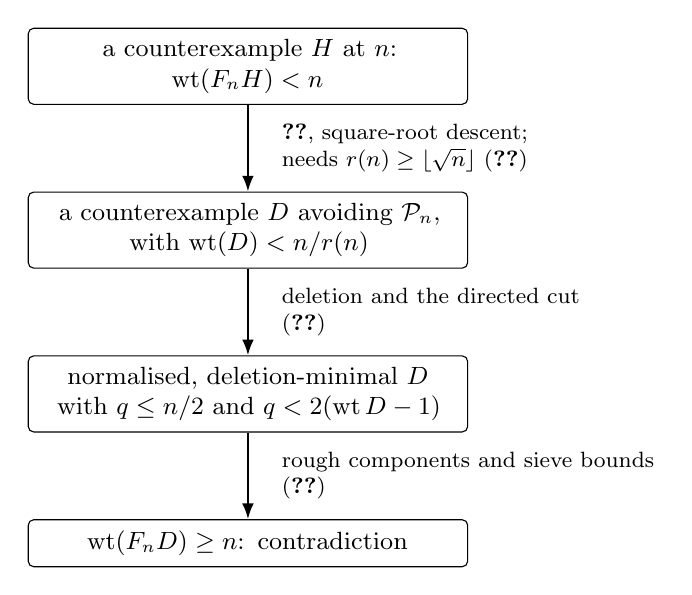
\begin{tikzpicture}[
  box/.style={draw,rounded corners=2pt,align=center,font=\small,inner sep=4pt,text width=5.3cm},
  node distance=11mm,
  arr/.style={-{Latex[length=2mm]},thick},
  lab/.style={font=\footnotesize,align=left}]
\node[box] (a) {a counterexample $H$ at $n$:\\ \mbox{$\wt(F_nH)<n$}};
\node[box,below=of a] (b) {a counterexample $D$ avoiding $\Pn$,\\ with \mbox{$\wt(D)<n/r(n)$}};
\node[box,below=of b] (c) {normalised, deletion-minimal $D$\\ with \mbox{$q\le n/2$} and \mbox{$q<2(\wt D-1)$}};
\node[box,below=of c] (d) {\mbox{$\wt(F_nD)\ge n$}: contradiction};
\draw[arr] (a)--(b) node[midway,right=3mm,lab]{\cref{thm:elimination}, square-root descent;\\ needs $r(n)\ge\lfloor\sqrt n\rfloor$ (\cref{prop:fresh-count})};
\draw[arr] (b)--(c) node[midway,right=3mm,lab]{deletion and the directed cut\\ (\cref{lem:directed-cut})};
\draw[arr] (c)--(d) node[midway,right=3mm,lab]{rough components and sieve bounds\\ (\cref{thm:localized-intro})};
\end{tikzpicture}
\caption{The proof of Theorem~A for a fixed $n\ge67$. No case $n'\ne n$ is used.}\label{fig:flow}
\end{figure}

The threshold $67$ is exactly where the counting hypothesis of the first move becomes available: $r(66)=7<8=\lfloor\sqrt{66}\rfloor$, while $r(n)\ge\lfloor\sqrt n\rfloor$ for all $n\ge67$. For $n\le66$ we apply the same descent directly with target~$n$. Explicit lower bounds for the cores $C_n$ show that any correction would be too expensive (\cref{sec:small}). Within that range, only the cases $n\le10$ are used as inputs to other cases.

\subsection{Relation to previous work}\label{sec:prior}
Several ingredients go back to Holdridge and Pach~\cite{HP}, and we indicate them where they are used.
\begin{itemize}
\item The ring structure of finite sets under $\triangle$ and $*$ and its identification with $\Ft[x_p]$ are in~\cite[Lemmas~2.1--2.2]{HP}. Polynomials over $\Ft$ also appear in the coding-theoretic origin of the problem~\cite{Pilz,PS} and in the proof of~\cite{NP}.
\item The decomposition by rough parts is~\cite[Lemma~2.4]{HP} (for $n$-rough parts). Slicing a multiplier by $p$-adic valuation is~\cite[Section~3]{HP}.
\item The fact that the primes in $(n/2,n]$ appear exactly once in $[n]$, and the importance of this fact, are emphasised in~\cite[Section~1]{HP}. Holdridge and Pach remove these primes one at a time. They expand the remaining multiplier in powers of $[n]\setminus\mathcal Q$ and use the identity $S*S=\{s^2:s\in S\}$~\cite[Lemma~6.2 and Section~6]{HP}. They also observe that, for products with $[n]\setminus T$, one may assume that no element of $A$ is divisible by a prime of $T$~\cite[proof of Lemma~6.1]{HP}. This is a precursor of \cref{cor:interval-elim}. Our square-root descent (\cref{sec:descent}) is an exact, threshold version of this mechanism. It removes all fresh primes at once, with no loss, as soon as there are $\lfloor\sqrt n\rfloor$ of them.
\item The splitting inequality of \cref{lem:directed-cut} is a variant of~\cite[Lemma~4.1 and Corollary~4.3]{HP}, combined here with minimality under deletion.
\item The lower bound through rough numbers in $(n/2,n]$ for smooth multipliers is~\cite[Lemma~4.4]{HP}. \Cref{thm:localized-intro} is an explicit refinement valid for every $n\ge67$.
\item The overall shape of the second and third moves follows Holdridge and Pach's proofs of their Theorem~1.4 and of the case $k\ge81$ of their Lemma~6.1. If a large prime divides an element of $A$, they split $A$ using~\cite[Corollary~4.3]{HP}. Otherwise $A$ is smooth, and they count rough numbers in $(n/2,n]$~\cite[Lemma~4.4]{HP}.
\item The identity $S*S=\{s^2:s\in S\}$ is~\cite[Lemma~6.2]{HP}. The pairing idea behind it goes back to the proof of~\cite[Theorem~5.1]{KM}.
\item The multiplicativity of weight parity is~\cite[Lemma~3.4]{HP}, generalising~\cite[Lemma~4]{Pilz}.
\item The two- and three-term cases of Theorem~A are due to Ke and Meyer~\cite{KM}. We reprove them in our framework because the small cases use them.
\item The example $\{1,2\}*\{1,2,4\}=\{1,8\}$, showing that Theorem~A fails for general $B$ in place of $[n]$, is from~\cite{HP}.
\end{itemize}
Holdridge and Pach used the explicit rough-number estimates of Fan and of Fan--Pomerance~\cite{Fan,FanPom} and the prime estimates of Rosser--Schoenfeld~\cite{RS}. To keep the present paper self-contained and suitable for formal verification, we instead prove the weaker estimates we need from first principles. These are Chebyshev's argument~\cite{Chebyshev} with the binomial-coefficient bound familiar from Erd\H{o}s's proof of Bertrand's postulate~\cite{Erdos} (see also~\cite{Hanson,Nair}), and a Legendre-type sieve for rough numbers in the sense of Buchstab~\cite{Buchstab}.

\subsection{Further results}
Besides Theorem~A, \cref{thm:elim-set} and \cref{thm:localized-intro}, the proof gives several statements of independent interest.
\begin{itemize}
\item Theorem~A holds over every field of characteristic two and for vector-valued multipliers (\cref{cor:char2}).
\item The polynomial elimination theorem (\cref{thm:elimination}) comes with a lower bound for every residual square class (\cref{prop:residual}).
\item Theorem~A holds for every multiplier with at most four terms, extending the case $|A|\le3$ of~\cite{KM}, and for every multiplier supported on at most three primes (\cref{cor:three-lists,thm:three-primes,cor:four-lists}). These are proved early, using only the cases $n\le10$.
\item Over any field, minimal counterexamples have a rigid structure: every element of their normalised support divides $(2u-3)!$, where $u$ is the number of terms (\cref{prop:factorial}). This is relevant to \cref{q:odd}.
\end{itemize}

\subsection{Organisation and notation}
\Cref{sec:prelim} sets up the polynomial model, the endpoint bound and the rough decomposition. \Cref{sec:descent} proves the elimination theorem, and \cref{sec:cut} the splitting inequality. \Cref{sec:assembly} assembles the proof for $n\ge67$ from two propositions, proved in \cref{sec:primes} (counting fresh primes) and \cref{sec:counting} (counting rough components). \Cref{sec:small} treats $n\le66$, and \cref{sec:remarks} discusses sharpness and open problems. \Cref{app:deps} records the logical dependencies, which we hope will be useful for formalisation.

Throughout, $p$ and $q$ denote primes, $\pi(t)$ is the number of primes at most $t$ (for real $t$), and $\log$ is the natural logarithm. \Cref{tab:notation} collects the main notation.

\begin{table}[ht]
\centering\small
\caption{Main notation.}\label{tab:notation}
\begin{tabular}{@{}ll@{}}
\toprule
$X(a)$, $F_n$ & monomial of $a\in\N$; $F_n=\sum_{a\le n}X(a)$\\
$\wt$, $\supp$, $\dist_\K$ & number of terms; support; minimal weight of a nonzero multiple\\
$\Pn$, $r(n)$ & fresh primes $p\in(n/2,n]$; $r(n)=|\Pn|=\pi(n)-\pi(n/2)$\\
$C_n$ & $F_n$ with the fresh terms removed\\
$\cl P\epsilon$, $\sigma(P)$ & full parity class of $P$; largest size of a parity class\\
$\sm jq$ & sum of $X(a)$ over $q$-smooth $a\le j$\\
$\Phi_q(t)$, $I_q(t)$ & number of $q$-rough $b\le t$; number of $q$-rough $b\in(t/2,t]$\\
$\varrho(q)$, $\delta_q$ & $\prod_{p\le q}(1-1/p)$; discrepancy bound for $\Phi_q$\\
$\width_x$, $W$ & $\deg_x-\ord_x$; total width in the base variables\\
\bottomrule
\end{tabular}
\end{table}

\section{The polynomial model}\label{sec:prelim}

\subsection{Encoding}
Let $\K$ be a field. We work in the polynomial ring $\K[x_p : p\text{ prime}]$ in one variable for each prime. Every polynomial involves only finitely many variables. Unique factorisation shows that $a\mapsto X(a)$ is a bijection from $\N$ onto the monomials, with $X(ab)=X(a)X(b)$. For finite $A,B\subset\N$ we therefore have, over $\Ft$,
\begin{equation}\label{eq:encoding}
 \Bigl(\sum_{a\in A}X(a)\Bigr)\Bigl(\sum_{b\in B}X(b)\Bigr)=\sum_{x\in A*B}X(x),
\end{equation}
since the coefficient of $X(x)$ on the left is the number of representations $x=ab$, reduced modulo~$2$. This is the identification of~\cite[Lemmas~2.1 and~2.2]{HP}. In particular $|A*[n]|=\wt(F_nH_A)$ with $H_A=\sum_{a\in A}X(a)$, and Theorem~A is equivalent to $\dist_{\Ft}(F_n)=n$. The upper bound $\dist_{\Ft}(F_n)\le n$ is witnessed by $H=1$.

For example, with $x=x_2$, $y=x_3$, $z=x_5$,
\[
 (1+x)(1+x+y+x^2+z+xy)=1+y+z+x^3+xz+x^2y,
\]
which records $\{1,2\}*[6]=\{1,3,5,8,10,12\}$.

We write $\supp P$ for the set of monomials of $P$ with nonzero coefficient. A nonzero polynomial is \emph{normalised} if its terms have no common monomial factor, that is, if its minimum exponent in every variable is zero. For a variable $x$, write $\deg_x P$ and $\ord_x P$ for the largest and smallest exponent of $x$ in $P$, and put $\width_x(P)=\deg_xP-\ord_xP$. Widths add under multiplication, since lowest and highest terms multiply.

\begin{lemma}[Elementary reductions]\label{lem:reductions}
Let $P\ne0$.
\begin{enumerate}[label=\textup{(\alph*)}]
\item Multiplying $P$ or a multiplier by a monomial changes neither weights nor $\dist_\K(P)$. In particular, multipliers may be assumed normalised.
\item If $P$ involves only the variables $\bx$, then $\dist_\K(P)$ is attained by a multiplier in $\K[\bx]$.
\item A nonzero multiple of a non-monomial has at least two terms.
\end{enumerate}
\end{lemma}

\begin{proof}
(a) is clear. For (b), let $H\ne0$ be any multiplier and expand $H=\sum_\beta \mathbf{w}^\beta H_\beta$ in the remaining variables $\mathbf{w}$, with $H_\beta\in\K[\bx]$. Then $PH=\sum_\beta\mathbf{w}^\beta(PH_\beta)$, and the summands have disjoint supports. Hence $\wt(PH_\beta)\le\wt(PH)$ for a nonzero $H_\beta$. For (c), a divisor of a monomial is a monomial.
\end{proof}

\subsection{Endpoints and parity}
The following bound is a polynomial form of the slicing by $p$-adic valuation used in~\cite[Section~3]{HP}.

\begin{lemma}[Endpoint bound]\label{lem:endpoints}
Let $y$ be a variable and $P=\sum_{i=0}^d a_iy^i$ with $d\ge1$, $a_0a_d\ne0$ and every $a_i$ independent of $y$. Then over any field
\[
                \dist(P)\ge\dist(a_0)+\dist(a_d).
\]
Consequently, if $P$ contains a nonzero constant term and a positive pure power of each of $s$ distinct variables, then $\dist(P)\ge s+1$. In particular $\dist(z_1+\cdots+z_r)\ge r$ and $\dist(1+z_1+\cdots+z_r)\ge r+1$.
\end{lemma}

\begin{proof}
Let $H\ne0$, and let $h_e$ and $h_f$ be the lowest and highest nonzero $y$-coefficients of $H$. The lowest and highest $y$-coefficients of $PH$ are $a_0h_e$ and $a_dh_f$. Both are nonzero, and they lie in different $y$-degrees because $d\ge1$. This proves the first claim.

For the second, slice in one of the $s$ variables. The lowest coefficient still contains the constant and the other $s-1$ pure powers. The highest coefficient is nonzero, so it has distance at least one. Induction on $s$ completes the proof.

For $z_1+\cdots+z_r$ the case $r=1$ is trivial. For $r\ge2$, slice in $z_1$: the lowest coefficient is $z_2+\cdots+z_r$ and the highest is $1$, so induction on $r$ applies. The bound for $1+z_1+\cdots+z_r$ is the second claim with $s=r$.
\end{proof}

\begin{lemma}[Weight parity~{\cite[Lemma~3.4]{HP}}]\label{lem:parity}
Over $\Ft$, $\wt(PH)\equiv\wt(P)\wt(H)\pmod 2$. In particular every multiple of a polynomial of even weight has even weight.
\end{lemma}

The special case that $|A*[n]|$ is even for even $n$ is~\cite[Lemma~4]{Pilz}.

\begin{proof}
Over $\Ft$, $\wt(P)\bmod2$ is the value of $P$ at $(1,1,\dots)$, and evaluation is a ring homomorphism.
\end{proof}

\subsection{Parity classes}
Over $\Ft$, the map $P\mapsto P^2$ is additive, and it sends distinct monomials to distinct monomials. Hence $\wt(P^2)=\wt(P)$. Every $P\in\Ft[\bx]$ has a unique decomposition
\begin{equation}\label{eq:parity}
  P=\sum_{\epsilon\in\{0,1\}^{\bx}}\bx^\epsilon\,P_\epsilon^2,
\end{equation}
obtained by grouping monomials according to the parities of their exponents. We call $\cl P\epsilon=\bx^\epsilon P_\epsilon^2$ the \emph{full parity class} of $P$ indexed by~$\epsilon$. Distinct classes have disjoint supports, and $\wt(\cl P\epsilon)=\wt(P_\epsilon)$. Let $\sigma(P)=\max_\epsilon\wt(\cl P\epsilon)$. In integer language, two monomials $X(a)$ and $X(b)$ lie in the same class exactly when $a$ and $b$ have the same squarefree part. Since every integer is uniquely a squarefree number times a square,
\begin{equation}\label{eq:squarefree-split}
 F_n=\sum_{\substack{a\le n\\ a\text{ squarefree}}} X(a)\,F_{\lfloor\sqrt{n/a}\rfloor}^{\,2}.
\end{equation}
Thus the class of $F_n$ indexed by a squarefree $a$ has $\lfloor\sqrt{n/a}\rfloor$ terms. Hence $\sigma(F_n)=\lfloor\sqrt n\rfloor$, attained by the squares, and every other class has at most $\lfloor\sqrt{n/2}\rfloor$ terms. The identity $F_n\cdot F_n=F_n^2$ is the polynomial form of $[n]*[n]=\{k^2:k\le n\}$~\cite{KM,HP}.

A polynomial all of whose exponents of a variable $z$ are even has formal derivative $\partial_zP=0$, and conversely. In characteristic two, $\partial_z(z^k)=kz^{k-1}$ is nonzero exactly when $k$ is odd. So $\partial_z$ maps each monomial that is odd in $z$ to a distinct monomial even in $z$, and kills the rest. Every derivative $\partial_zP$ is even in~$z$.

\subsection{Rough components}\label{sec:rough}
Let $T$ be a finite set of primes. An integer is \emph{$T$-smooth} if all its prime factors lie in $T$, and \emph{$T$-rough} if none does. For real $t\ge0$ and integers $j\ge1$ put
\[
 F_j^{(T)}=\sum_{\substack{a\le j\\ a\ T\text{-smooth}}}X(a),\qquad
 \Phi_T(t)=\#\{b\le t:\ b\ T\text{-rough}\},\qquad
 I_T(t)=\Phi_T(t)-\Phi_T(t/2).
\]
Thus $I_T(t)$ counts the $T$-rough integers in $(t/2,t]$. When $T$ is the set of primes at most $q$, we say \emph{$q$-smooth} and \emph{$q$-rough}, and write $\sm jq$, $\Phi_q$ and $I_q$.

Each $a\le n$ factors uniquely as $a=bc$ with $b$ $T$-rough and $c$ $T$-smooth. A multiplier $D$ involving only primes in $T$ preserves the $T$-rough part of every monomial. Hence (compare~\cite[Lemma~2.4]{HP})
\begin{equation}\label{eq:rough-decomposition}
 F_nD=\sum_{\substack{b\le n\\ b\ T\text{-rough}}}X(b)\,F^{(T)}_{\lfloor n/b\rfloor}D,
 \qquad
 \wt(F_nD)=\sum_{\substack{b\le n\\ b\ T\text{-rough}}}\wt\bigl(F^{(T)}_{\lfloor n/b\rfloor}D\bigr),
\end{equation}
over any field. The summands have pairwise disjoint supports. We call $F^{(T)}_{\lfloor n/b\rfloor}D$ the \emph{component} of $b$, and $\lfloor n/b\rfloor$ its \emph{index}. For each $k\ge1$ there are exactly $\Phi_T(n/k)$ components of index at least~$k$. There are $I_T(n)$ components of index one, and each of them is a copy of~$D$.

\begin{lemma}[Component profile]\label{lem:profile}
Let $D$ be a normalised nonconstant polynomial over any field, and let $q$ be the largest prime whose variable occurs in $D$. Then for every $j\ge1$,
\[
 \wt\bigl(\sm jq D\bigr)\ \ge\
 \begin{cases}
 \wt(D) & j=1,\\
 2\bigl(1+\pi(j)\bigr) & 2\le j<q,\\
 1+\pi(q) & j\ge q.
 \end{cases}
\]
\end{lemma}

\begin{proof}
For $j=1$ the component is $D$. If $2\le j<q$, then $\sm jq=F_j$ is independent of $x_q$. Since $D$ is normalised and involves $x_q$, it has at least two nonzero $x_q$-slices. Multiplication by $F_j$ keeps these slices in distinct $x_q$-degrees. Each product contains a nonzero multiple of $F_j$, and $F_j$ contains $1$ and the variables $x_p$ for $p\le j$, so each has at least $1+\pi(j)$ terms by \cref{lem:endpoints}. If $j\ge q$, then $\sm jq$ contains $1$ and $x_p$ for every $p\le q$, and \cref{lem:endpoints} gives $1+\pi(q)$.
\end{proof}

Summing the profile over components gives two budgets that we use repeatedly. Every component of index at least two has at least four terms if $q\ge5$. Moreover, the profile values at indices $1,2,3,4$ and at every index $\ge5$ are at least $\wt(D),4,6,6,8$ when $q\ge17$, because $\pi(17)=7$. Writing $u=\wt(D)$, we obtain
\begin{align}
 \wt(F_nD)&\ge 4\Phi_q(n)+(u-4)I_q(n) && (q\ge5),\label{eq:budget4}\\
 \wt(F_nD)&\ge u\,I_q(n)+4\Phi_q(n/2)+2\Phi_q(n/3)+2\Phi_q(n/5) && (q\ge17).\label{eq:budget8}
\end{align}
Inequality~\eqref{eq:budget4} holds for every $u\ge1$, since $u$ is the exact weight of each index-one component. The lower bound through the index-one components alone, $\wt(F_nD)\ge u\,I_q(n)$, is the bound of~\cite[Lemma~4.4]{HP}.

\section{Eliminating the fresh primes}\label{sec:descent}

All polynomials in this section have coefficients in $\Ft$.

\subsection{Setting}
Fix base variables $\bx=(x_1,\dots,x_t)$ and fresh variables $\bz=(z_1,\dots,z_r)$ with $r\ge1$. Let $0\ne C\in\Ft[\bx]$ and put
\[
 Z=z_1+\cdots+z_r,\qquad F=C+Z.
\]
By \cref{lem:reductions}(b) we may compute $\dist(F)$ inside $\Ft[\bx,\bz]$. A polynomial is \emph{fresh-even} if it lies in $\Ft[\bx,z_1^2,\dots,z_r^2]$. Only base variables enter the total width
\[
 W(P)=\sum_{i=1}^t\width_{x_i}(P)\qquad(P\ne0).
\]
For a variable $x_i$, the width of $F$ equals $\deg_{x_i}C$, because $Z$ has $x_i$-exponent $0$. Hence
\begin{equation}\label{eq:widthF}
 \width_{x_i}(F)=\deg_{x_i}C\qquad(1\le i\le t).
\end{equation}
Fix an integer target $N$ with $1\le N\le\wt(C)+r$. Call a nonzero multiple $G$ of $F$ \emph{short} if $\wt(G)<N$.

\begin{definition}[Extremal multiples]\label{def:extremal}
A short multiple $G$ of $F$ is \emph{extremal} if it minimises $W$ among all short multiples, and minimises $\wt$ among the short multiples with that value of $W$.
\end{definition}

Extremal multiples exist whenever short ones do, because $W$ and $\wt$ take values in $\N\cup\{0\}$. The descent consists of replacing an extremal multiple by others that are still extremal, until it takes a rigid form.

\begin{lemma}[Basic facts]\label{lem:basic}
\begin{enumerate}[label=\textup{(\alph*)}]
\item $F$ is a prime element of $\Ft[\bx,\bz]$. It divides no monomial, it does not divide $Z$, and it does not divide $z_i+z_j$ for $i\ne j$.
\item If $\wt(C)=1$, there are no short multiples. Hence, if short multiples exist, then $C$ is not a monomial and $W(F)\ge1$.
\item \textup{(Stability.)} Let $G$ be extremal and let $G'$ be a nonzero multiple of $F$ with $\wt(G')\le\wt(G)$ and $\width_{x_i}(G')\le\width_{x_i}(G)$ for all $i$. Then $G'$ is extremal, with the same weight and the same widths as~$G$.
\item If $G$ is extremal and $\bz^\beta$ is a monomial in the fresh variables, then $\bz^\beta G$ is extremal.
\item For $i\ne j$ the derivation $\partial_{ij}=\partial_{z_i}+\partial_{z_j}$ satisfies $\partial_{ij}F=0$. Hence $\partial_{ij}(FH)=F\,\partial_{ij}H$, and $\partial_{ij}$ maps multiples of $F$ to multiples of $F$. Every $\partial_{z_i}$ maps a polynomial to one whose base exponents occur among those of the original.
\end{enumerate}
\end{lemma}

\begin{proof}
(a) Since $F$ is linear in $z_1$ with coefficient $1$, substituting $z_1=C+z_2+\cdots+z_r$ identifies $\Ft[\bx,\bz]/(F)$ with the domain $\Ft[\bx,z_2,\dots,z_r]$. So $F$ is prime, and $F$ divides a polynomial exactly when that polynomial vanishes under the substitution. A monomial maps to a nonzero product, since $C+z_2+\cdots+z_r\ne0$. The polynomial $Z$ maps to $C\ne0$. For $i,j\ne1$, $z_i+z_j$ maps to itself. Finally $z_1+z_j$ maps to $C+\sum_{k\ne1,j}z_k$, which is nonzero because $C\ne0$ involves no fresh variable.

(b) If $C=\bx^\alpha$ is a monomial, then $\dist(F)\ge r+1=\wt(C)+r\ge N$. This follows by slicing $F=\bx^\alpha+z_1+\cdots+z_r$ successively in $z_1,\dots,z_r$ as in \cref{lem:endpoints}. Otherwise $C$ involves some $x_i$, and $W(F)\ge\deg_{x_i}C\ge1$ by~\eqref{eq:widthF}.

(c) $G'$ is short, so $W(G')\ge W(G)$ by extremality. Since each width of $G'$ is at most the corresponding width of $G$, all widths are equal. Extremality then gives $\wt(G')\ge\wt(G)$, hence equality.

(d) Multiplying by $\bz^\beta$ changes neither base widths nor weight.

(e) $\partial_{z_i}F=1$ for every $i$. The rest is the Leibniz rule and the fact that $\partial_{z_i}$ does not change base exponents.
\end{proof}

Note that $\wt(\partial_{z_i}G)$ equals the number $m_i(G)$ of terms of $G$ whose $z_i$-exponent is odd.

\subsection{Synchronising the fresh rows}

\begin{proposition}[Synchronised normal form]\label{prop:normal-form}
Suppose short multiples of $F$ exist. Then there is an extremal multiple $G$, of weight $m$ say, with
\[
 G=G_0+Z D,\qquad m=\wt(G_0)+r\,u,\qquad u:=\wt(D)\le\tfrac m2,
\]
where $G_0$ and $D$ are fresh-even and nonzero.
In particular $ru<m<N$, and $\partial_{z_i}G=D$ for every $i$.
\end{proposition}

\begin{proof}
By \cref{lem:basic}(b), $W(F)\ge1$. Start from any extremal $G$, of weight $m$, and write $m_i=m_i(G)$.

\emph{Step 1 (parity normalisation).} Multiplying by $z_i$ replaces $m_i$ by $m-m_i$ and leaves the other $m_j$ unchanged. By \cref{lem:basic}(d) we may therefore assume $m_i\le m/2$ for all~$i$.

\emph{Step 2 (synchronisation).} Suppose that $m_i<m/2$ for some $i$, and let $j\ne i$. By \cref{lem:basic}(e), $\partial_{ij}G$ is a multiple of $F$ of weight at most $m_i+m_j<m$, with no larger base widths than $G$. By \cref{lem:basic}(c) it must vanish. Hence all the derivatives $\partial_{z_j}G$ coincide; call the common value~$D$. Since $D=\partial_{z_j}G$ is even in $z_j$ for every $j$, it is fresh-even. Put $G_0=G+ZD$. Then
\[
 \partial_{z_j}G_0=D+(\partial_{z_j}Z)D+Z\,\partial_{z_j}D=D+D+0=0
\]
for every $j$, so $G_0$ is fresh-even. In $G=G_0+ZD$ the summands $G_0$, $z_1D,\dots,z_rD$ have pairwise disjoint supports: $G_0$ is even in every fresh variable, while $z_jD$ is odd in $z_j$ only. Hence $m=\wt(G_0)+r\,\wt(D)$ and $u=\wt(D)=m_i\le m/2$. If $r=1$, Step 2 applies without any condition on $m_1$: it is just the decomposition by $z_1$-parity.

\emph{Step 3 (the balanced case).} Suppose $r\ge2$ and $m_i=m/2$ for every $i$. Write $y=z_1$, $y'=z_2$ and
\[
 G=B_{00}+yB_{10}+y'B_{01}+yy'B_{11},
\]
with each $B_{kl}$ even in $y$ and $y'$. The conditions $m_1=m_2=m/2$ give $\wt(B_{10})=\wt(B_{01})=:b$ and $\wt(B_{00})=\wt(B_{11})=:h$ with $m=2(h+b)$.

If $b>0$, put $G'=\partial_{12}G=B_{10}+B_{01}+(y+y')B_{11}$. This is a multiple of $F$ of weight at most $2b+2h=m$, with no larger base widths. It is nonzero. Indeed, $G'=0$ would force $B_{11}=0$, hence $h=0$ and $B_{00}=0$, and $B_{10}=B_{01}$, so $G=(y+y')B_{10}$. Then $F\mid B_{10}$ by \cref{lem:basic}(a), and $B_{10}$ is a nonzero multiple of weight $m/2<m$ with no larger widths, contradicting \cref{lem:basic}(c). So $G'$ is extremal by \cref{lem:basic}(c), and its number of terms odd in $y$ is $\wt(B_{11})=h<m/2$.

If $b=0$, put $G''=\partial_{12}(yG)=B_{00}+y^2B_{11}$. Here $yG$ is extremal by \cref{lem:basic}(d). If $G''=0$ then $G=y(y+y')B_{11}$, and the same argument gives a contradiction. So $G''$ is extremal, and it has no terms odd in $y$.

In both cases we obtain an extremal multiple with $m_1<m/2$. Multiplying by suitable $z_j$ with $j\ge3$ restores $m_j\le m/2$ for those $j$ without changing $m_1$, and Step 2 applies.

\emph{Step 4 ($D\ne0$).} Let $G$ be as produced by Step 2, and suppose $D=0$, so that every fresh derivative of $G$ vanishes. Write $G=FH$. Then $0=\partial_{z_1}G=H+F\,\partial_{z_1}H$, so $F\mid H$ and $G=F^2E$. Since $F^2$ is fresh-even and $\partial_{z_j}G=F^2\partial_{z_j}E$, the polynomial $E$ is fresh-even. Decompose it as $E=\sum_{\epsilon}\bx^{\epsilon}E_\epsilon^2$ over base parities. Then
\[
 G=\sum_\epsilon \bx^\epsilon (FE_\epsilon)^2,
\]
and the summands have disjoint supports. Choose $\epsilon$ with $E_\epsilon\ne0$. Then $FE_\epsilon$ is a nonzero multiple of $F$ of weight $\wt(\bx^\epsilon(FE_\epsilon)^2)\le m<N$. Its widths satisfy $2\width_{x_i}(FE_\epsilon)=\width_{x_i}(\bx^\epsilon(FE_\epsilon)^2)\le\width_{x_i}(G)$. Since $W(G)\ge W(F)\ge1$, we get $W(FE_\epsilon)\le W(G)/2<W(G)$, contradicting extremality.

\emph{Step 5 ($G_0\ne0$).} If $r=1$, then $m=\wt(G_0)+u$ and $u\le m/2$ force $\wt(G_0)\ge m/2>0$. If $r\ge2$ and $G_0=0$, then $G=ZD$. Since $F$ is prime and does not divide $Z$, we get $F\mid D$. But $D=\partial_{z_1}G$ is nonzero, has weight $m/r<m$, and has no larger widths than $G$, contradicting \cref{lem:basic}(c).

Finally $G_0\ne0$ gives $ru<m$.
\end{proof}

\subsection{The residual and its square classes}

\begin{proposition}[Residual classes cost the full target]\label{prop:residual}
Let $G=G_0+ZD$ be as in \cref{prop:normal-form}, and put
\[
 R=G+FD=G_0+CD.
\]
Then $R$ is fresh-even and divisible by $F^2$, and every nonzero full parity class of $R$ has at least $N$ terms.
\end{proposition}

\begin{proof}
The two expressions for $R$ agree because $ZD+ZD=0$. The second shows that $R$ is fresh-even. Write $G=FH$. Then $D=\partial_{z_1}G=H+F\,\partial_{z_1}H$, so $R=FH+FH+F^2\partial_{z_1}H=F^2J$ with $J=\partial_{z_1}H$. Since $R$ is fresh-even and $\partial_{z_j}R=F^2\partial_{z_j}J$, the polynomial $J$ is fresh-even too.

If $R=0$, the assertion is immediate; assume $R\ne0$.

\emph{The cofactor $H$ has positive width in some base variable.} Otherwise $H=\bx^\beta H'$ with $H'\in\Ft[\bz]$. Let $c_0\in\{0,1\}$ be the constant term of $C$. Then $FH'=(C-c_0)H'+(c_0+Z)H'$. The terms of $(C-c_0)H'$ are copies of $H'$ in distinct nonzero base monomials, and $(c_0+Z)H'$ lies in base degree zero. By \cref{lem:endpoints},
\[
 \wt(FH')=(\wt(C)-c_0)\wt(H')+\wt((c_0+Z)H')\ge \wt(C)-c_0+r+c_0\ge N,
\]
contradicting $\wt(FH')=\wt(G)<N$.

\emph{Width of the residual.} Fix a base variable $x$. Every exponent of $x$ in $G_0$ or in $D=\partial_{z_1}G$ is an exponent of $x$ in $G$. Since $R=G_0+CD$, we get $\ord_xR\ge\ord_xG$ and $\deg_xR\le\deg_xG+\deg_xC$. Using~\eqref{eq:widthF} and $\width_x(G)=\width_x(F)+\width_x(H)$, this gives
\begin{equation}\label{eq:residual-width}
 \width_x(R)\le\width_x(G)+\width_x(F)=2\width_x(G)-\width_x(H).
\end{equation}

\emph{Square classes.} Since $R=F^2J$ is fresh-even, decomposing $J$ by full parity shows that the nonzero full parity classes of $R$ are $\cl R\epsilon=\bx^\epsilon(FJ_\epsilon)^2$ for base parity vectors $\epsilon$ and polynomials $J_\epsilon$. Here $\wt(\cl R\epsilon)=\wt(FJ_\epsilon)$, and by~\eqref{eq:residual-width}
\[
 \width_x(FJ_\epsilon)=\tfrac12\width_x(\cl R\epsilon)\le\tfrac12\width_x(R)\le\width_x(G)-\tfrac12\width_x(H)
\]
for every base variable $x$, with strict inequality for at least one~$x$. Thus $FJ_\epsilon$ is a nonzero multiple of $F$ with $W(FJ_\epsilon)<W(G)$. By extremality it is not short, so $\wt(\cl R\epsilon)=\wt(FJ_\epsilon)\ge N$.
\end{proof}

The polynomial $G$ differs from the multiple $FD$ only by $R$. The fresh-odd part of $FD$ is $ZD$ and its fresh-even part is $CD$. A residual class can therefore be cancelled only by the corresponding class of $CD$. This yields the following comparison. Let $a$ denote the number of nonzero full parity classes of~$R$.

\begin{corollary}[Protected classes]\label{cor:protection}
In the situation of \cref{prop:residual}:
\begin{enumerate}[label=\textup{(\roman*)}]
\item If $\wt(\cl{(CD)}\epsilon)<ru+N-m$, then $\cl R\epsilon=0$. In particular this holds whenever $\wt(\cl{(CD)}\epsilon)\le ru$.
\item If every full parity class of $CD$ has at most $M$ terms, then
\[
 m\ge\wt(FD)+a(N-2M)\qquad\text{and}\qquad a(N-M)\le m-ru .
\]
\item Let $M$ bound every class of $CD$. If either $N\ge2M$ and $\wt(FD)\ge N$, or $a\le1$ and $\wt(FD)\ge\max\{N,2M\}$, then $m\ge N$, which is impossible. In applications this shows that no short multiple exists.
\end{enumerate}
\end{corollary}

\begin{proof}
Classwise, $\cl G\epsilon=\cl R\epsilon+\cl{(FD)}\epsilon$. Every class of $R$ is fresh-even, and for fresh-even $\epsilon$ we have $\cl{(FD)}\epsilon=\cl{(CD)}\epsilon$. Moreover $\cl G\epsilon$ is then contained in $G_0$, whose weight is $m-ru$. If $\cl R\epsilon\ne0$, then
\[
 m-ru\ge\wt(\cl G\epsilon)\ge N-\wt(\cl{(CD)}\epsilon),
\]
which proves~(i). For (ii), each $\epsilon$ with $\cl R\epsilon\ne0$ satisfies
\[
 \wt(\cl G\epsilon)\ge N-M\ge\wt(\cl{(FD)}\epsilon)+N-2M.
\]
The other classes satisfy $\wt(\cl G\epsilon)=\wt(\cl{(FD)}\epsilon)$. Summing over all classes gives the first inequality. The $a$ classes with $\cl R\epsilon\ne0$ lie in $G_0$, which gives the second. For~(iii): in the first case $m\ge\wt(FD)\ge N$. In the second, $m\ge\wt(FD)\ge N$ if $a=0$, and $m\ge\wt(FD)+N-2M\ge N$ if $a=1$.
\end{proof}

\subsection{The elimination theorem}

\begin{theorem}[Fresh-variable elimination]\label{thm:elimination}
If $r\ge\sigma(C)$, then
\[
 \dist(C+z_1+\cdots+z_r)=\min_{0\ne D\in\Ft[\bx]}\bigl(\wt(CD)+r\,\wt(D)\bigr).
\]
In particular, the minimum on the left is attained by a multiplier involving no fresh variable.
\end{theorem}

\begin{proof}
Let $d$ denote the right-hand side. A multiplier $D\in\Ft[\bx]$ gives $FD=CD+z_1D+\cdots+z_rD$ with disjoint summands, so $\dist(F)\le d\le\wt(C)+r$ (take $D=1$). Suppose $\dist(F)<d$. Then short multiples exist for the target $N=d$, and \cref{prop:normal-form} provides $G=G_0+ZD$ with fresh-even $D\ne0$ of weight $u$.

Every full parity class of $CD$ is a sum of products $\cl C{\epsilon'}\cdot\cl D{\epsilon''}$ with $\epsilon'+\epsilon''\equiv\epsilon$. For fixed $\epsilon$, each class of $D$ occurs once, so the class has at most $\sigma(C)\,u\le ru$ terms. By \cref{cor:protection}(i), $R=0$, that is, $G=FD$.

Write $D=\sum_\alpha \bz^{2\alpha}D_\alpha$ with $D_\alpha\in\Ft[\bx]$. Then
\[
 G=FD=\sum_\alpha\Bigl(\bz^{2\alpha}CD_\alpha+\sum_{i=1}^r\bz^{2\alpha}z_iD_\alpha\Bigr).
\]
All these summands have pairwise disjoint supports, since their fresh exponent vectors are $2\alpha$ and $2\alpha+e_i$. Hence
\[
 m=\wt(G)=\sum_\alpha\bigl(\wt(CD_\alpha)+r\,\wt(D_\alpha)\bigr)\ge d,
\]
because some $D_\alpha\ne0$. This contradicts $m<N=d$.
\end{proof}

\begin{proof}[Proof of \cref{thm:elim-set}]
Let $\bx$ be the variables of the primes dividing elements of $B_0$, and let $z_p=x_p$ for $p\in T$. By hypothesis $\sum_{b\in B}X(b)=C+\sum_{p\in T}z_p$ with $C=\sum_{b\in B_0}X(b)\in\Ft[\bx]$. Two elements of $B_0$ lie in the same square class exactly when their monomials lie in the same full parity class, so $\sigma(C)=\sigma(B_0)$.

If $B_0=\emptyset$, so that $B=T$, both sides equal $|T|$ by \cref{lem:endpoints}. So let $B_0\ne\emptyset$; then $|T|\ge\sigma(B_0)\ge1$. By~\eqref{eq:encoding}, the left-hand side of the theorem is $\dist(C+\sum_{p\in T}z_p)$, which may be computed in $\Ft[\bx,\bz]$ by \cref{lem:reductions}(b). By \cref{thm:elimination} it equals the minimum of $\wt(CD)+|T|\wt(D)$ over nonzero $D\in\Ft[\bx]$.

On the right-hand side, $A$ may involve further primes outside $T$. Let $\mathbf w$ be the corresponding variables and let $D$ be free of the $z_p$. Expanding $D=\sum_\beta\mathbf w^\beta D_\beta$ with $D_\beta\in\Ft[\bx]$ gives $\wt(CD)+|T|\wt(D)=\sum_\beta\bigl(\wt(CD_\beta)+|T|\wt(D_\beta)\bigr)$. So such primes never lower the minimum. Finally, for $A$ with no element divisible by a prime of $T$, the encoding gives $\wt(CH_A)=|A*B_0|$ and $\wt(H_A)=|A|$.
\end{proof}

\begin{example}[The hypothesis $r\ge\sigma(C)$ is needed]\label{ex:sharp}
Let $x=x_2$, $z=x_3$ and $C=(1+x)^5=1+x+x^4+x^5$, so that $\sigma(C)=2$ and $r=1$. In integers, $B=\{1,2,3,16,32\}$, $T=\{3\}$ and $B_0=\{1,2,16,32\}$. Then
\[
 G=(1+x)z^3+1+x^{16}=(C+z)\,(1+x)(z^2+Cz+C^2)
\]
has four terms. With the corresponding $A$,
\[
 A=\{1,2,3,4,8,9,12,18,48,192,256,512,1024,2048\},
\]
we get $A*B=\{1,27,54,65536\}$. On the other hand, every $D\in\Ft[x]\setminus\{0\}$ has $\wt(CD)+\wt(D)\ge5$. For one-term $D$ the value is $5$, and for $D$ with at least three terms it is at least $2+3$. For two terms we may take $D=1+x^j$ with $j\ge1$; then the exponent set $\{0,1,4,5\}$ of $C$ meets its translate by $j$ in at most two points, so $\wt(CD)\ge4$. As in the proof of \cref{thm:elim-set}, further primes cannot lower this minimum, so $|A*B_0|+|A|\ge5$ for every nonempty $A$ coprime to $3$. So the conclusion of \cref{thm:elim-set} fails for $B=\{1,2,3,16,32\}$.

The multiple $G$ also shows the structure described in \cref{prop:normal-form,prop:residual}. With target $N=5$, it has the synchronised form with $m=4$, $D=(1+x)z^2$, $u=2$, $G_0=1+x^{16}$ and $R=F^2(1+x)^6$. The residual has a single parity class, of weight $6\ge N$, as \cref{prop:residual} requires of extremal multiples. (We have not proved that $G$ is extremal.) The matching class of $CD$ has weight $4>ru+N-m=3$, so it is not protected, and the cancellation is genuine.
\end{example}

\subsection{Application to intervals}
For $F_n$ the fresh variables are $x_p$ with $p\in\Pn$, and $F_n=C_n+Z_n$ with $Z_n=\sum_{p\in\Pn}x_p$. Removing these primes from $[n]$ leaves every square. So, by~\eqref{eq:squarefree-split}, $\sigma(C_n)=\lfloor\sqrt n\rfloor$.

\begin{corollary}[Counterexamples avoid the fresh primes]\label{cor:interval-elim}
Let $n\ge2$ with $r(n)\ge\lfloor\sqrt n\rfloor$. If $\dist_{\Ft}(F_n)<n$, then there is a nonzero $D$ involving only the primes at most $n/2$ with
\[
 \wt(F_nD)=\wt(C_nD)+r(n)\wt(D)<n.
\]
In particular $\wt(D)<n/r(n)$.
\end{corollary}

\begin{proof}
By \cref{lem:reductions}(b) we may work with the variables of $F_n$. These are the base variables $x_p$ with $p\le n/2$ and the fresh variables. Now apply \cref{thm:elimination}.
\end{proof}

\begin{corollary}[Characteristic two and vector coefficients]\label{cor:char2}
Let $\K$ be a field of characteristic two, or let $V$ be a vector space over $\Ft$. If Theorem~A holds for a given $n$, then $\wt(F_nH)\ge n$ for every nonzero finitely supported $H=\sum_a h_aX(a)$ with coefficients in $\K$, respectively in $V$. Here weight counts monomials with nonzero coefficient.
\end{corollary}

\begin{proof}
The coefficients of $H$ span a finite-dimensional $\Ft$-space. Choose an $\Ft$-linear functional $\lambda$ on it that does not vanish on all of them. Applying $\lambda$ coefficientwise commutes with multiplication by $F_n$, because $F_n$ has coefficients in $\Ft$. It also cannot enlarge supports. So $\wt(F_nH)\ge\wt(F_n\lambda(H))\ge n$.
\end{proof}

\section{Minimal counterexamples and the directed cut}\label{sec:cut}

Fix $n\ge1$ and a field $\K$. A nonzero $H\in\K[x_p]$ is a \emph{counterexample at $n$} if $\wt(F_nH)<n$. It is \emph{minimal under deletion} if no polynomial obtained by deleting some, but not all, of its terms is a counterexample. Every counterexample contains one that is minimal under deletion: keep deleting terms while a counterexample remains. Deletion never introduces a new variable, so it preserves any restriction on the primes involved. Dividing by the greatest common monomial factor also preserves minimality under deletion, by \cref{lem:reductions}(a).

The next lemma is a variant of the splitting inequality of Holdridge and Pach~\cite[Lemma~4.1 and Corollary~4.3]{HP}. Here the split is taken at a prime power, intersections are counted from the lower side only, and the input is minimality under deletion.

\begin{lemma}[Directed cut]\label{lem:directed-cut}
Let $D$ be a normalised counterexample at $n$ that is minimal under deletion, with $u$ terms, and let $q$ be a prime. For $a\ge0$ let $u_a$ be the number of terms of $D$ whose $x_q$-exponent equals $a$. Then for every $b>0$ with $u_b>0$,
\begin{equation}\label{eq:directed-cut}
 2\sum_{a<b}u_a\left\lfloor\frac{n}{q^{\,b-a}}\right\rfloor>n.
\end{equation}
Consequently every prime $q$ whose variable occurs in $D$ satisfies
\[
                    q<2u_0\le2(u-1).
\]
\end{lemma}

\begin{proof}
Split $D=L+U$, where $L$ consists of the terms with $x_q$-exponent less than $b$. Both pieces are nonzero (the exponent $0$ is occupied because $D$ is normalised), so both are proper. Minimality gives $\wt(F_nL)\ge n$ and $\wt(F_nU)\ge n$. Over any field,
\[
 \wt(P+Q)\ge\wt(P)+\wt(Q)-2\,|\supp P\cap\supp Q|,
\]
so $n>\wt(F_nD)$ forces $|\supp(F_nL)\cap\supp(F_nU)|>n/2$.

Every monomial of $F_nU$ has $x_q$-exponent at least $b$. A monomial of $F_nL$ with $x_q$-exponent at least $b$ arises from a term of $L$ with exponent $a<b$ and an integer $j\le n$ with $q^{b-a}\mid j$. There are $\lfloor n/q^{b-a}\rfloor$ such $j$. Hence the intersection has at most $\sum_{a<b}u_a\lfloor n/q^{b-a}\rfloor$ elements, proving~\eqref{eq:directed-cut}.

If $x_q$ occurs in $D$, let $b$ be its least positive exponent. Then only $a=0$ contributes, and $2u_0\lfloor n/q^b\rfloor>n$ gives $q\le q^b<2u_0$. Finally $u_0\le u-1$ because the exponent $b$ is occupied.
\end{proof}

A more general form of this inequality, which counts all gaps between occupied exponents, is given in \cref{sec:remarks}. It shows that the support of a minimal counterexample consists of divisors of $(2u-3)!$.

\section{Proof of Theorem A for \texorpdfstring{$n\ge67$}{n >= 67}}\label{sec:assembly}

The proof for $n\ge67$ uses two counting statements, proved in the next two sections.

\begin{proposition}[Fresh primes]\label{prop:fresh-count}
For every integer $n\ge67$ we have $r(n)\ge\lfloor\sqrt n\rfloor$. Moreover:
\begin{enumerate}[label=\textup{(\alph*)}]
\item for $67\le n\le1023$, $r(n)\ge8$ and
\[
 \beta(n):=10\,r(n)+4\pi(n/2)+2\pi(n/3)+2\pi(n/5)-48\ \ge\ n;
\]
\item for $1024\le n\le32768$, $r(n)>n/30$;
\item for $n\ge32768$, $r(n)>7n/(20\log n)$.
\end{enumerate}
\end{proposition}

The value $67$ is optimal for the first assertion: $r(66)=7<8=\lfloor\sqrt{66}\rfloor$.

The second statement is \cref{thm:localized-intro} from the introduction. We prove it in \cref{sec:counting}. It holds over every field, and it assumes no minimality of~$D$.

\begin{proof}[Proof of Theorem~A for $n\ge67$]
Fix $n\ge67$ and suppose that $\dist_{\Ft}(F_n)<n$. By \cref{prop:fresh-count}, $r(n)\ge\lfloor\sqrt n\rfloor$. So \cref{cor:interval-elim} provides a counterexample at $n$ involving only primes at most $n/2$. Delete terms until it is minimal under deletion, and divide by its greatest common monomial factor. Call the result $D$, with $u$ terms. Both operations preserve the restriction to primes at most $n/2$ and the property of being a counterexample.

A monomial multiplier gives exactly $n$ terms, so $D$ is not a monomial. Let $q$ be the largest prime whose variable occurs in $D$. Then $q\le n/2$, and \cref{lem:directed-cut} gives $q<2(u-1)$. Now \cref{thm:localized-intro} gives $\wt(F_nD)\ge n$, contradicting the choice of~$D$.
\end{proof}

\begin{remark}
The argument works at a single fixed $n$. It uses no instance of Theorem~A at any other interval length, and in particular no induction on~$n$.
\end{remark}

\section{Counting the fresh primes}\label{sec:primes}

This section proves \cref{prop:fresh-count}. For $n\le1023$ we compute directly from the residues modulo~$30$. For larger $n$ we use an elementary form of Chebyshev's method.

\subsection{From \texorpdfstring{$67$}{67} to \texorpdfstring{$100$}{100}}

\begin{lemma}\label{lem:67-100}
For $67\le n\le100$ we have $r(n)\ge8+\mathbf 1_{n\ge73}+\mathbf 1_{n\ge97}\ge\lfloor\sqrt n\rfloor$ and $\beta(n)\ge104\ge n$.
\end{lemma}

\begin{proof}
An integer in $(33,100]$ coprime to $30$ is prime unless it is divisible by $7$, since every composite number up to $100$ has a prime factor at most~$7$. The integers in $(33,100]$ coprime to $30$ are
\[
 37,\,41,\,43,\,47,\,49,\,53,\,59,\,61,\,67,\,71,\,73,\,77,\,79,\,83,\,89,\,91,\,97,
\]
and removing $49$, $77$ and $91$ leaves the primes. At $n=67$ the fresh primes are $37,41,43,47,53,59,61,67$, so $r(67)=8$. As $n$ runs from $67$ to $100$:
\begin{itemize}
\item a prime enters $(n/2,n]$ at $n=71,73,79,83,89,97$;
\item a prime leaves it at $n=74,82,86,94$.
\end{itemize}
Pair the arrivals $71,79,83,89$ with the departures $74,82,86,94$, respectively. Each arrival precedes its departure, and $73$ and $97$ remain unpaired. This proves the bound for $r(n)$. The comparison with $\lfloor\sqrt n\rfloor$ holds because $\lfloor\sqrt n\rfloor\le8$ for $n\le80$, $\lfloor\sqrt n\rfloor=9$ for $81\le n\le99$, and $\lfloor\sqrt{100}\rfloor=10$.

The primes up to $33$ are $2,3,\dots,31$, eleven in number. So $\pi(n/2)\ge\pi(33)=11$, $\pi(n/3)\ge\pi(22)=8$ and $\pi(n/5)\ge\pi(13)=6$ throughout the range. Hence $\beta(n)\ge80+44+16+12-48=104$.
\end{proof}

\subsection{From \texorpdfstring{$101$}{101} to \texorpdfstring{$1023$}{1023}}
Let $\mathcal R=\{1,7,11,13,17,19,23,29\}$ be the residues coprime to $30$. For real $x\ge0$ write $\lfloor x\rfloor=30h+s$ with $0\le s<30$, and put
\[
 N_{30}(x)=8h+\#\{a\in\mathcal R:a\le s\},
\]
the number of positive integers at most $x$ coprime to $30$. Let $\Phi_7(x)=N_{30}(x)-N_{30}(x/7)$ count the $7$-rough integers up to~$x$.

\begin{lemma}[An exact prime count below $1024$]\label{lem:semiprime}
Let $(p_1,\dots,p_7)=(11,13,17,19,23,29,31)$. For every real $x$ with $7\le x\le1023$,
\[
 \pi(x)=3+\Phi_7(x)-\sum_{i=1}^{7}\max\{\Phi_7(x/p_i)-i,\,0\}.
\]
\end{lemma}

\begin{proof}
A $7$-rough integer up to $1023$ is $1$, a prime greater than $7$, or a product of two primes greater than $7$, because $11^3=1331>1023$. In a product $pp'$ with $p\le p'$ we have $p\le\sqrt{1023}<32$, so $p=p_i$ for some~$i$. For fixed $p_i$, the admissible $p'$ are the primes in $[p_i,x/p_i]$. Since $x/p_i\le93<121=11^2$, every $7$-rough integer up to $x/p_i$ is $1$ or a prime. Exactly $i$ of them, namely $1,p_1,\dots,p_{i-1}$, lie below $p_i$. So there are $\max\{\Phi_7(x/p_i)-i,0\}$ such products. Each composite is counted once, prime squares included. Adding the primes $2,3,5,7$ and removing the integer $1$ gives the formula.
\end{proof}

\begin{proposition}\label{prop:101-1023}
For $101\le n\le1023$ we have $r(n)\ge\lfloor\sqrt n\rfloor$ and $\beta(n)\ge n$.
\end{proposition}

\begin{proof}
Cover $[101,1023]$ by the thirteen intervals $[a,b]$ of \cref{tab:low-range}. For $n\in[a,b]$, monotonicity gives
\[
 r(n)\ge r_0:=\pi(a)-\pi(b/2),
 \qquad
 \beta(n)\ge\beta_0:=10r_0+4\pi(a/2)+2\pi(a/3)+2\pi(a/5)-48 .
\]
It therefore suffices that $r_0\ge\lfloor\sqrt b\rfloor$ and $\beta_0\ge b$ in each row, which the table shows. All prime counts follow from \cref{lem:semiprime}.

For instance, in the row $[422,524]$, the five arguments $422$, $262$, $211$, $140$, $84$ (integer parts of $a$, $b/2$, $a/2$, $a/3$, $a/5$) give the following.
\begin{itemize}
\item $N_{30}$ values: $113,70,57,38,23$; at $x/7$: $16,10,8,6,3$.
\item $\Phi_7$ values: $97,60,49,32,20$.
\item Correction sums: $18,8,5,1,0$. For $x=422$ the seven corrections are $8,6,3,1,0,0,0$.
\item Prime counts: $82,55,47,34,23$.
\end{itemize}
Hence $r_0=27\ge22$ and $\beta_0=270+188+68+46-48=524=b$.
\end{proof}

\begin{table}[ht]
\centering\small
\caption{Prime counts for $101\le n\le1023$.}\label{tab:low-range}
\setlength{\tabcolsep}{4pt}
\begin{tabular}{rr|rrrrr|rrr}
\toprule
$a$&$b$&$\pi(a)$&$\pi(b/2)$&$\pi(a/2)$&$\pi(a/3)$&$\pi(a/5)$&$r_0$&$\lfloor\sqrt b\rfloor$&$\beta_0$\\\midrule
101&117&26&16&15&11&8&10&10&150\\
118&141&30&19&17&12&9&11&11&172\\
142&165&34&22&20&15&9&12&12&200\\
166&195&38&25&23&16&11&13&13&228\\
196&225&44&29&25&18&12&15&15&262\\
226&273&48&32&30&21&14&16&16&302\\
274&345&58&39&33&24&16&19&18&354\\
346&421&68&46&40&30&19&22&20&430\\
422&524&82&55&47&34&23&27&22&524\\
525&636&99&66&55&40&27&33&25&636\\
637&765&115&75&66&47&31&40&27&772\\
766&913&135&87&76&54&36&48&30&916\\
914&1023&156&97&88&62&42&59&31&1102\\\bottomrule
\end{tabular}
\end{table}

\subsection{An elementary Chebyshev estimate}
Let $\vartheta(x)=\sum_{p\le x}\log p$ and $\psi(x)=\sum_{p^k\le x}\log p$. We use Chebyshev's combination of factorials~\cite{Chebyshev} together with the bound $\lcm(1,\dots,k)<4^k$, which goes back to the central-binomial argument in Erd\H{o}s's proof of Bertrand's postulate~\cite{Erdos}; see also~\cite{Hanson,Nair}. Put
\[
 \mu_1=\frac{14\log2+9\log3+5\log5}{30},\qquad \mu_2=\frac65\mu_1,\qquad
 \eta(x)=\frac{5}{4\log6}\Bigl(\log x+\tfrac12\log6-\tfrac65\Bigr)^2+9 .
\]

\begin{lemma}[Elementary Chebyshev bounds]\label{lem:chebyshev}
For $x\ge30$,
\[
 \mu_1x-\tfrac52\log x+2<\psi(x)<\mu_2x+\eta(x),
\]
and for $x\ge256$,
\[
 0\le\psi(x)-\vartheta(x)<\tfrac83\sqrt x .
\]
Consequently, for $n\ge256$,
\begin{equation}\label{eq:rlogn}
 r(n)\log n>\tfrac25\mu_1n-\tfrac83\sqrt n-\tfrac52\log n+2-\eta(n/2).
\end{equation}
\end{lemma}

\begin{proof}
Write $\lambda(t)=\log\lfloor t\rfloor!$ and $h(t)=t\log t-t$.

\emph{Factorials.} We first show, for $t\ge1$,
\begin{equation}\label{eq:stirling}
 h(t)-\tfrac12\log t+\tfrac{1+\log2}2\le\lambda(t)\le h(t)+\tfrac12\log t+1 .
\end{equation}
For an integer $k\ge1$, the trapezoidal rule underestimates $\int_1^k\log v\,dv=h(k)+1$ by concavity, so $\lambda(k)\le h(k)+\frac12\log k+1$. This extends to real $t$ since $h$ and $\log$ increase on $[1,\infty)$. For the lower bound, concavity gives $\log i\ge\int_{i-1/2}^{i+1/2}\log v\,dv$. Summing over $i\le k=\lfloor t\rfloor$ gives
\[
 \lambda(t)\ge h(k+\tfrac12)-h(\tfrac12)=h(k+\tfrac12)+\tfrac{1+\log2}{2}.
\]
Finally $h(t)-h(k+\frac12)\le\frac12\log t$, because $h'=\log$ and $t<k+1$.

\emph{Chebyshev's combination.} Put
\[
 \Xi(x)=\lambda(x)-\lambda(x/2)-\lambda(x/3)-\lambda(x/5)+\lambda(x/30).
\]
In the combination of the functions $h(x/d)$, the coefficients of $x\log x$ and of $x$ vanish. The remaining linear term is $\mu_1x$. Applying~\eqref{eq:stirling} to each term, for $x\ge30$,
\begin{equation}\label{eq:Xi}
 \mu_1x-\tfrac52\log x+\log60-2\ \le\ \Xi(x)\ \le\ \mu_1x+\tfrac52\log x-\log30+\tfrac{1-3\log2}{2}.
\end{equation}
The numerical bounds below give $\log60-2>2$ and $-\log30+\frac{1-3\log2}2<-3$.

By Legendre's formula $\lambda(x)=\sum_{p^k\le x}\lfloor x/p^k\rfloor\log p$, we have
\[
 \Xi(x)=\sum_{p^k\le x}f(x/p^k)\log p,\qquad f(t)=\lfloor t\rfloor-\lfloor t/2\rfloor-\lfloor t/3\rfloor-\lfloor t/5\rfloor+\lfloor t/30\rfloor .
\]
The function $f$ has period $30$ and is constant on each interval $[k,k+1)$. In one period it equals $1$ on the intervals with left endpoint
\[
 1,2,3,4,5,7,8,9,11,13,14,17,19,23,29,
\]
and $0$ elsewhere. In particular $0\le f\le1$, and $f=1$ on $[1,6)$. Hence
\[
 \psi(x)-\psi(x/6)\le\Xi(x)\le\psi(x),
\]
and the lower bound for $\psi$ follows from~\eqref{eq:Xi}.

\emph{The bound $\psi(t)<t\log4$ for $t\ge1$.} Equivalently, $\lcm(1,\dots,k)<4^k$ for every integer $k\ge1$. We induct on $k$; the case $k=1$ is clear. Passing from $k-1$ to an even $k$ multiplies the lcm by at most $2$, because the only prime power that can be even is a power of~$2$. For $k=2m+1$, every prime power $p^e\in(m+1,2m+1]$ with $p^{e-1}\le m+1$ contributes a single factor $p$. That $p$ divides $\binom{2m+1}{m}$, by Legendre's formula at the level $p^e$. Hence
\[
 \lcm(1,\dots,2m+1)\le\lcm(1,\dots,m+1)\binom{2m+1}{m}<4^{m+1}4^m ,
\]
using $2\binom{2m+1}{m}\le2^{2m+1}$.

\emph{Upper bound for $\psi$.} Iterate $\psi(x)\le\Xi(x)+\psi(x/6)$ until $t=x/6^k\in[5,30)$. Each argument $x/6^j$ with $j<k$ is at least $30$, so~\eqref{eq:Xi} applies. The linear terms sum to $\mu_2(x-t)$. Moreover $\psi(t)<t\log4$ and $(\log4-\mu_2)t<9$. The logarithmic terms sum to
\[
 \sum_{j=0}^{k-1}\Bigl(\tfrac52(\log x-j\log6)-3\Bigr)
 =-\tfrac54\log6\,k^2+\Bigl(\tfrac52\log x+\tfrac54\log6-3\Bigr)k\le\eta(x)-9,
\]
by completing the square.

\emph{Prime powers.} Grouping even exponents,
\[
 \psi(x)-\vartheta(x)=\psi(\sqrt x)+\sum_{\substack{a\ge3\\ a\text{ odd}}}\vartheta(x^{1/a}).
\]
At most $\frac{\log x}{2\log2}-\frac32$ odd exponents $a\ge5$ contribute. With $\psi(t)<t\log4$ this gives
\[
 \frac{\psi(x)-\vartheta(x)}{\sqrt x}<\log4\Bigl(1+x^{-1/6}+\bigl(\tfrac{\log x}{2\log2}-\tfrac32\bigr)x^{-3/10}\Bigr).
\]
For $x\ge256$ we have $x^{-1/6}<\frac25$. The last term decreases for $x\ge256$, because $\log2>\frac23$, and at $x=256$ it equals $\frac52\cdot2^{-12/5}<\frac12$. Since $\log4<\frac75$, the bound is less than $\frac75\cdot\frac{19}{10}<\frac83$.

\emph{Conclusion.} Every prime in $(n/2,n]$ contributes at most $\log n$ to $\vartheta(n)-\vartheta(n/2)$, so $r(n)\log n\ge\vartheta(n)-\vartheta(n/2)$. Insert the bounds above, noting that $\mu_1n-\frac12\mu_2n=\frac25\mu_1n$.

\emph{Numerical constants.} All logarithm bounds used come from the series $\log\frac{1+t}{1-t}=2\sum_{j\ge0}t^{2j+1}/(2j+1)$.
\begin{itemize}
\item The first three terms at $t=\frac13$ give $\log2>\frac{693}{1000}$. Bounding the remaining denominators below by $3$ gives $\log2<\frac{25}{36}<\frac7{10}$.
\item The first four terms at $t=\frac12$ give $\log3>\frac{1098}{1000}$.
\item The first two terms at $t=\frac19$ give $\log\frac54>\frac{223}{1000}$, hence $\log5>\frac{1609}{1000}$.
\item The same tail bound at $t=\frac15$ gives $\log\frac32<\frac{73}{180}$.
\end{itemize}
These give $\mu_1>\frac{23}{25}$ and $\log6>\frac{25}{14}$, so $\frac{5}{4\log6}<\frac7{10}$. They also give $\log2+\frac65-\frac12\log6=\frac65-\frac12\log\frac32>\frac{99}{100}$, as well as the two constants used for~\eqref{eq:Xi}.
\end{proof}

\subsection{Large \texorpdfstring{$n$}{n}}

\begin{lemma}\label{lem:fresh-large}
We have $r(n)>n/30$ for $1024\le n\le32768$ and $r(n)>7n/(20\log n)$ for $n\ge32768$. In particular $r(n)>\sqrt n$ for all $n\ge1024$.
\end{lemma}

\begin{proof}
Put $L=\log n$ and
\[
 w(L)=\tfrac7{10}\bigl(L-\tfrac{99}{100}\bigr)^2+\tfrac52L+7,\qquad
 g(L)=\tfrac{46}{125}-\tfrac83e^{-L/2}-e^{-L}w(L).
\]
For $L>6$, the constants at the end of the proof of \cref{lem:chebyshev} give
\[
 \eta(n/2)=\tfrac5{4\log6}\Bigl(L-\bigl(\log2+\tfrac65-\tfrac12\log6\bigr)\Bigr)^2+9<\tfrac7{10}\bigl(L-\tfrac{99}{100}\bigr)^2+9 .
\]
Together with $\mu_1>\frac{23}{25}$, inequality~\eqref{eq:rlogn} then yields $r(n)L/n>g(L)$.

For $L\ge6$, $g$ is increasing and strictly concave. Indeed $g'=\frac43e^{-L/2}+e^{-L}(w-w')$ and $g''=-\frac23e^{-L/2}-e^{-L}(w-2w'+w'')$, and both
\[
 w-w'=\tfrac7{10}\Bigl\{\bigl(L-\tfrac{99}{100}\bigr)^2-2\bigl(L-\tfrac{99}{100}\bigr)\Bigr\}+\tfrac52L+\tfrac92
\]
and
\[
 w-2w'+w''=\tfrac7{10}\Bigl\{\bigl(L-\tfrac{299}{100}\bigr)^2-2\Bigr\}+\tfrac52L+2
\]
are positive there. Hence $g(L)-L/30$ is strictly concave as well.

\emph{The endpoint $n=1024$.} Here $L<7$, $\sqrt n=32$ and $w(7)<50$, so
\[
 g(L)-\tfrac L{30}>\tfrac{46}{125}-\tfrac1{12}-\tfrac{50}{1024}-\tfrac7{30}=\tfrac{481}{192000}>0 .
\]
\emph{The endpoint $n=32768=2^{15}$.} Here $L<\frac{21}2$, $\sqrt n>180$ and $w(\frac{21}2)<97$, so
\[
 g(L)-\tfrac7{20}>\tfrac{46}{125}-\tfrac2{135}-\tfrac{97}{32768}-\tfrac7{20}=\tfrac{24881}{110592000}>0 .
\]
At $n=32768$ also $L/30<\frac7{20}$. By concavity, $g(L)>L/30$ on the whole first range, which gives $r(n)>n/30$. Since $g$ is increasing, $g(L)>\frac7{20}$ on the second range, which gives $r(n)>7n/(20\log n)$.

Finally, $n/30>\sqrt n$ for $n\ge1024$. The function $\sqrt n/\log n$ increases for $n\ge e^2$, and $\frac7{20}\cdot\frac{180}{21/2}=6>1$, so $7n/(20\log n)>\sqrt n$ for $n\ge32768$.
\end{proof}

\begin{proof}[Proof of \cref{prop:fresh-count}]
Combine \cref{lem:67-100}, \cref{prop:101-1023} and \cref{lem:fresh-large}. The bound $r(n)\ge8$ for $n\le1023$ follows from the first two.
\end{proof}

\section{Counting rough components}\label{sec:counting}

This section proves \cref{thm:localized-intro}. Throughout, $\K$ is any field and $D\in\K[x_p]$ is normalised and nonconstant, with $u$ terms and largest prime~$q$. All estimates rest on~\eqref{eq:rough-decomposition}, \cref{lem:profile} and the budgets \eqref{eq:budget4}--\eqref{eq:budget8}, in which every coefficient is nonnegative (for~\eqref{eq:budget4}, as soon as $u\ge4$, which holds whenever we use it). So lower bounds for the counts $\Phi_q$ and $I_q$ may be substituted directly.

\subsection{Sieve estimates}
Put $\varrho(q)=\prod_{p\le q}(1-1/p)$.

\begin{lemma}[Discrepancy]\label{lem:discrepancy}
For every real $x\ge0$, $|\Phi_q(x)-\varrho(q)x|\le \delta_q$, where
\[
 \delta_2=\tfrac12,\qquad \delta_3=\tfrac23,\qquad \delta_q=\tfrac{14}{15}\,2^{\pi(q)-3}\quad(q\ge5).
\]
Consequently $I_q(x)\ge\varrho(q)x/2-2\delta_q$.
\end{lemma}

\begin{proof}
The cases $q=2,3$ follow from the residues modulo $2$ and $6$. Modulo $30$ the rough residues are $\mathcal R=\{1,7,11,13,17,19,23,29\}$. At these points the values of $15\Phi_5(x)-4x$ are
\[
 11,\ 2,\ 1,\ 8,\ 7,\ 14,\ 13,\ 4 .
\]
Between consecutive jumps the error $\Phi_5(x)-\frac4{15}x$ decreases linearly. Just before the jump at a listed point it equals the listed value divided by $15$, minus one. The error is periodic modulo $30$, so $|\Phi_5(x)-\frac4{15}x|\le\frac{14}{15}$. Adding a prime $p$ to the sieve gives $\Phi_{T\cup\{p\}}(x)=\Phi_T(x)-\Phi_T(x/p)$. This multiplies the density by $1-1/p$ and at most doubles the discrepancy. Induction proves the claim, and subtracting the estimates at $x$ and $x/2$ gives the bound for~$I_q$.
\end{proof}

\begin{lemma}[A one-step sieve]\label{lem:one-step}
Let $T$ and $T'$ be disjoint finite sets of primes, and suppose $|\Phi_T(x)-\varrho x|\le \delta$ for all $x\ge0$. Put
\[
 \alpha=\varrho\Bigl(1-\sum_{p\in T'}\frac1p\Bigr),\qquad \bar\delta=(1+|T'|)\,\delta .
\]
Then $\Phi_{T\cup T'}(x)\ge\alpha x-\bar\delta$ and $I_{T\cup T'}(x)\ge\alpha x/2-2\bar\delta$. If moreover $|I_T(x)-\varrho x/2|\le \delta'$ for all $x$, then $I_{T\cup T'}(x)\ge\alpha x/2-(1+|T'|)\delta'$.
\end{lemma}

\begin{proof}
Remove from the $T$-rough integers the multiples of each $p\in T'$, charging an integer once for each such divisor. Since multiplication by $p\notin T$ preserves $T$-roughness, this union bound gives
\[
 \Phi_{T\cup T'}(x)\ge\Phi_T(x)-\sum_{p\in T'}\Phi_T(x/p).
\]
The same argument on $(x/2,x]$ gives $I_{T\cup T'}(x)\ge I_T(x)-\sum_{p\in T'}I_T(x/p)$. Insert the discrepancy bounds, using $\delta'=2\delta$ when no better bound is available.
\end{proof}

\begin{lemma}[Half-interval discrepancy]\label{lem:half}
For every real $x\ge0$, $|I_5(x)-\frac2{15}x|\le\frac{22}{15}$.
\end{lemma}

\begin{proof}
The error $I_5(x)-\frac{2}{15}x$ has period $60$, since $I_5(x+60)=I_5(x)+8$. Between jumps it has slope $-\frac2{15}$. It jumps up at the integers coprime to~$30$ and down at twice those integers. At the sixteen upward jumps $t\in(0,60)$ the values of $15I_5(t)-2t$ are:

\smallskip
\begin{center}\small
\begin{tabular}{c|rrrrrrrr}
$t$&1&7&11&13&17&19&23&29\\\hline
$15I_5(t)-2t$&13&1&8&19&11&22&14&2\\[2pt]
$t$&31&37&41&43&47&49&53&59\\\hline
$15I_5(t)-2t$&13&1&$-7$&4&$-4$&7&14&2
\end{tabular}
\end{center}
\smallskip

So the error is at most $\frac{22}{15}$. For nonintegral $x\in(0,60)$, the reflection $b\mapsto60-b$ of residues gives $I_5(60-x)=8-I_5(x)$, so the error changes sign. Every value is a one-sided limit of values at nonintegral points, which proves the lower bound.
\end{proof}

For a prime $q\ge7$ put
\[
 \alpha_q=\tfrac4{15}\Bigl(1-\sum_{7\le p\le q}\tfrac1p\Bigr),\qquad \nu_q=\pi(q)-2 .
\]
\Cref{lem:discrepancy,lem:one-step,lem:half}, applied with $T=\{2,3,5\}$ and $|T'|=\pi(q)-3$, give
\begin{equation}\label{eq:alpha-sieve}
 \Phi_q(x)\ge\alpha_qx-\tfrac{14}{15}\nu_q,\qquad I_q(x)\ge\tfrac12\alpha_qx-\tfrac{22}{15}\nu_q .
\end{equation}

\subsection{Small support primes}

\begin{proposition}\label{prop:small-q}
\Cref{thm:localized-intro} holds when $q\le13$.
\end{proposition}

\begin{proof}
Let $n\ge67$. The hypothesis $q<2(u-1)$ gives $u\ge3,4,5,7,8$ for $q=3,5,7,11,13$, respectively.

\emph{$q=2$.} Every component has at least two terms (\cref{lem:profile}), so $\wt(F_nD)\ge2\Phi_2(n)=2\lceil n/2\rceil\ge n$.

\emph{$q=3$.} The profile is $u\ge3$ at index one, $4$ at index two (as $2<q$), and $3$ beyond. Hence
\[
 \wt(F_nD)\ge3\Phi_3(n)+\bigl(\Phi_3(n/2)-\Phi_3(n/3)\bigr).
\]
The residues $1,5$ modulo $6$ give $3\Phi_3(n)\ge n-1$. Consecutive such residues are at most $4$ apart, so the interval $(n/3,n/2]$, of length $n/6\ge4$, contains a $3$-rough integer.

\emph{$q=5$.} Every component has at least four terms, so
\[
 \wt(F_nD)\ge4\Phi_5(n)\ge\tfrac{16n-56}{15}\ge n\qquad(n\ge56).
\]

\emph{$q=7,11,13$.} With the least admissible $u$, the profile from index two onwards is bounded below by
\[
 (4,5,5,\dots),\qquad(4,6,6,\dots),\qquad(4,6,6,7,7,\dots),
\]
respectively. Hence $\wt(F_nD)\ge\Lambda_q(n)$, where
\begin{align*}
 \Lambda_7(n)&=5\Phi_7(n)-\Phi_7(n/2)+\Phi_7(n/3)=4\Phi_7(n)+I_7(n)+\Phi_7(n/3),\\
 \Lambda_{11}(n)&=7\Phi_{11}(n)-3\Phi_{11}(n/2)+2\Phi_{11}(n/3)=4\Phi_{11}(n)+3I_{11}(n)+2\Phi_{11}(n/3),\\
 \Lambda_{13}(n)&=8\Phi_{13}(n)-4\Phi_{13}(n/2)+2\Phi_{13}(n/3)+\Phi_{13}(n/5)\\
 &=4\Phi_{13}(n)+4I_{13}(n)+2\Phi_{13}(n/3)+\Phi_{13}(n/5).
\end{align*}
Larger values of $u$ only add $(u-u_{\min})I_q(n)\ge0$. Substitute into the second, nonnegative forms the bounds $\Phi_q(x)\ge\alpha_qx-\frac{14}{15}\nu_q$ from~\eqref{eq:alpha-sieve} and $I_q(x)\ge\frac12\alpha_qx-2\cdot\frac{14}{15}\nu_q$ from \cref{lem:one-step}, with the constants
\[
\begin{array}{c|ccc}
q&7&11&13\\\hline
\alpha_q&8/35&236/1155&184/1001\\
\tfrac{14}{15}\nu_q&28/15&14/5&56/15
\end{array}
\]
For these three primes the cruder error $2\cdot\frac{14}{15}\nu_q$ in the bound for $I_q$ is sufficient, so we use it rather than $\frac{22}{15}\nu_q$ from~\eqref{eq:alpha-sieve}. This gives
\[
 \Lambda_7(n)\ge\tfrac{116n-1372}{105},\qquad
 \Lambda_{11}(n)\ge\tfrac{4366n-116424}{3465},\qquad
 \Lambda_{13}(n)\ge\tfrac{18952n-840840}{15015}.
\]
Since weights are integers, these give $\wt(F_nD)\ge n$ as soon as the right side exceeds $n-1$. This happens for $n\ge116$, $126$, $210$ respectively, the conditions being $11n>1267$, $901n>112959$ and $3937n>825825$.

For the remaining ranges we use \cref{tab:small-q}. For a row $[a,b]$ put $b_7=\min(b,115)$, $b_{11}=\min(b,125)$ and $b_{13}=b$. Since $\Phi_q$ is nondecreasing, $\Lambda_q(n)\ge\Lambda^-_q$ for $a\le n\le b_q$. Here $\Lambda^-_q$ is obtained from the first form of $\Lambda_q$ by replacing every positive argument $n/k$ by $a/k$, and the sole negative argument $n/2$ by $b_q/2$. Every entry is at least the corresponding $b_q$. A dash means that the linear bound already covers the row.

\begin{table}[ht]
\centering\small
\caption{Lower bounds $\Lambda^-_q$ for $67\le n\le209$.}\label{tab:small-q}
\begin{tabular}{c|rrr}
\toprule
$[a,b]$&$\Lambda^-_7$&$\Lambda^-_{11}$&$\Lambda^-_{13}$\\\midrule
$[67,76]$&76&89&91\\
$[77,85]$&86&102&105\\
$[86,94]$&94&110&114\\
$[95,101]$&101&121&127\\
$[102,110]$&110&132&139\\
$[111,145]$&126&149&149\\
$[146,181]$&--&--&181\\
$[182,209]$&--&--&238\\\bottomrule
\end{tabular}
\end{table}

The counts in \cref{tab:small-q} come from $N_{30}$ (\cref{sec:primes}) by inclusion--exclusion over the primes $7,11,13$. For $0\le t\le209$,
\begin{align*}
 \Phi_7(t)&=N_{30}(t)-N_{30}(t/7),\\
 \Phi_{11}(t)&=N_{30}(t)-N_{30}(t/7)-N_{30}(t/11)+\mathbf 1_{t\ge77},\\
 \Phi_{13}(t)&=N_{30}(t)-N_{30}(t/7)-N_{30}(t/11)-N_{30}(t/13)+\mathbf 1_{t\ge77}+\mathbf 1_{t\ge91}+\mathbf 1_{t\ge143}.
\end{align*}
These hold because $t/(pp')<7$ for distinct $p,p'\in\{7,11,13\}$, so that $N_{30}(t/(pp'))=\mathbf 1_{t\ge pp'}$, and because $7\cdot11\cdot13=1001>209$. For example, in the row $[111,145]$ the values of $\Phi_q$ at $111$, at $b_q/2$, at $37$ and at $111/5$ are $(26,13,9,5)$, $(25,14,8,4)$ and $(24,15,7,3)$ for $q=7,11,13$. The three bounds are therefore $130-13+9=126$, $175-42+16=149$ and $192-60+14+3=149$.
\end{proof}

\subsection{Larger support primes up to \texorpdfstring{$n=1023$}{n = 1023}}

\begin{lemma}[Prime budget]\label{lem:prime-budget}
Suppose $r(n)\ge8$, $17\le q\le n/2$ and $q<2(u-1)$. Then
\[
 \wt(F_nD)\ge\beta(n)+(u-10)(r(n)-8)\ge\beta(n),
\]
with $\beta(n)$ as in \cref{prop:fresh-count}.
\end{lemma}

\begin{proof}
Every prime in $(n/2,n]$ exceeds $q$, so $I_q(n)\ge r(n)$. Also $\Phi_q(t)\ge1+\pi(t)-\pi(q)$ for all $t$: when the right side is positive, it counts $1$ and the primes in $(q,t]$. Inserting these into~\eqref{eq:budget8} gives
\[
 \wt(F_nD)\ge u\,r(n)+4\pi(n/2)+2\pi(n/3)+2\pi(n/5)+8-8\pi(q).
\]
Now $q\le2u-3$, and $u\ge10$ since $q\ge17$. Increasing $u$ by one adds a single odd integer to $[1,2u-3]$, so $\pi(q)\le\pi(2u-3)\le\pi(17)+(u-10)=u-3$. Substituting gives the claim.
\end{proof}

\subsection{Larger support primes beyond \texorpdfstring{$n=1023$}{n = 1023}}

\begin{lemma}[Reciprocal sums]\label{lem:reciprocals}
We have
\[
 \sum_{7\le p\le53}\frac1p<\frac{259}{400},\qquad
 \sum_{11\le p\le149}\frac1p<\frac{229}{320},\qquad
 \sum_{11\le p\le271}\frac1p<\frac{33}{40}.
\]
\end{lemma}

\begin{proof}
Since $\sqrt{271}<17$, an integer in $[17,271]$ is prime exactly when it is coprime to $2\cdot3\cdot5\cdot7\cdot11\cdot13$. So the primes in $[17,271]$ are the integers there that are coprime to $30$ and not divisible by $7$, $11$ or $13$. Together with $11$ and $13$, they are the primes in $[11,271]$. Let $B_j$ be the sum of $1/p$ over these primes in $[30j,30j+30)$. Then:

\smallskip
\begin{center}\small
\begin{tabular}{c|l|r}
$j$&denominators in $B_j$&$4000B_j<$\\\hline
0&11, 13, 17, 19, 23, 29&1429\\
1&31, 37, 41, 43, 47, 53, 59&657\\
2&61, 67, 71, 73, 79, 83, 89&381\\
3&97, 101, 103, 107, 109, 113&230\\
4&127, 131, 137, 139, 149&147\\
5&151, 157, 163, 167, 173, 179&146\\
6&181, 191, 193, 197, 199&105\\
7&211, 223, 227, 229, 233, 239&106\\
8&241, 251, 257, 263, 269&79\\
9&271&15
\end{tabular}
\end{center}
\smallskip

The first sum is less than $\frac17+\frac{1429+657}{4000}-\frac1{59}=\frac{259}{400}-\frac{19}{206500}$. The second and third are less than $\frac{2844}{4000}=\frac{711}{1000}<\frac{229}{320}$ and $\frac{3295}{4000}=\frac{659}{800}<\frac{33}{40}$.
\end{proof}

\begin{lemma}[{Support primes in $[17,53]$}]\label{lem:five-bands}
If $17\le q\le53$ and $q<2(u-1)$, then $\wt(F_nD)>n$ for every $n\ge1024$.
\end{lemma}

\begin{proof}
By~\eqref{eq:budget8} (in the equivalent form $4\Phi_q(n)+(u-4)I_q(n)+2\Phi_q(n/3)+2\Phi_q(n/5)$) and~\eqref{eq:alpha-sieve},
\begin{equation}\label{eq:five-band}
 \wt(F_nD)\ge\alpha_q\Bigl(\frac u2+\frac{46}{15}\Bigr)n-\frac{22u+24}{15}\,\nu_q .
\end{equation}
Use the five bands below. In each band, $u\ge u_*$, $\nu_q\le\nu_*$ and $\alpha_q>a_*$. The last inequality follows from the first sum in \cref{lem:reciprocals}, after removing the primes beyond the band.
\[
\begin{array}{c|ccccc}
q\in&[17,23]&[29,37]&[41,43]&\{47\}&\{53\}\\\hline
u_*&10&16&22&25&28\\
a_*&7/50&7/60&13/125&99/1000&47/500\\
\nu_*&7&10&12&13&14
\end{array}
\]
At $n=1024$ and $u=u_*$, the right side of~\eqref{eq:five-band}, with $a_*$ and $\nu_*$ in place of $\alpha_q$ and $\nu_q$, exceeds $n$ by
\[
 \tfrac{6964}{375},\quad\tfrac{10672}{225},\quad\tfrac{126832}{1875},\quad\tfrac{106162}{1875},\quad\tfrac{40192}{1875}.
\]
At $n=1024$ its slopes in $u$ are $\frac{4606}{75}$, $\frac{676}{15}$, $\frac{4456}{125}$, $\frac{11858}{375}$, $\frac{10348}{375}$. Its slope in $n$, minus one, is positive at $u_*$ and increases with $u$. So the bound exceeds $n$ for all $n\ge1024$ and $u\ge u_*$.
\end{proof}

\begin{lemma}[{Support primes in $[59,271]$}]\label{lem:middle}
If $59\le q\le271$ and $q<2(u-1)$, then $\wt(F_nD)>n$ for every $n\ge32768$.
\end{lemma}

\begin{proof}
Sieve first by $T_0=\{2,3,5,7\}$. This has density $\frac8{35}$ and discrepancy at most $\frac{28}{15}$ by \cref{lem:discrepancy}. With
\[
 \alpha=\tfrac8{35}\Bigl(1-\sum_{11\le p\le q}\tfrac1p\Bigr),\qquad \bar\delta=\tfrac{28}{15}\bigl(\pi(q)-3\bigr),
\]
\cref{lem:one-step} and~\eqref{eq:budget4} give
\[
 \wt(F_nD)\ge4(\alpha n-\bar\delta)+(u-4)(\tfrac12\alpha n-2\bar\delta)=\tfrac{u+4}2\alpha n-2(u-2)\bar\delta .
\]
From $\pi(q)\le2+\Phi_5(q)<3+\frac{4q}{15}$ we get $\bar\delta<\frac{112q}{225}$.
\begin{itemize}
\item If $59\le q\le149$, then \cref{lem:reciprocals} gives $\alpha>\frac{13}{200}$, and $\bar\delta<75$, and the hypothesis gives $u\ge31$. At $n=32768$ and $u=31$ the bound minus $n$ is $\frac{11}{80}\cdot32768-2\cdot29\cdot75=\frac{778}5>0$.
\item If $151\le q\le271$, then $\alpha>\frac1{25}$, $\bar\delta<135$ and $u\ge77$. The corresponding margin is $\frac{31}{50}\cdot32768-2\cdot75\cdot135=\frac{1654}{25}>0$.
\end{itemize}
In both cases the slopes in $n$ and in $u$ are positive at the corner and remain so; the $u$-slopes are $\frac{13}{400}n-150$ and $\frac{n}{50}-270$.
\end{proof}

\begin{lemma}[Odd-integer telescoping]\label{lem:rho}
For every odd prime $q$, $\varrho(q)>1/(2\sqrt q)$.
\end{lemma}

\begin{proof}
Including the odd composite factors decreases the product. For odd $m\ge3$ we have $(1-1/m)^2>(m-2)/m$, and the product of $(m-2)/m$ over odd $m\in[3,q]$ telescopes to $1/q$. Hence $\varrho(q)\ge\frac12\prod_{3\le m\le q,\ m\text{ odd}}(1-1/m)>\frac1{2\sqrt q}$.
\end{proof}

By Mertens' theorem~\cite{Mertens}, $\varrho(q)\sim e^{-\gamma}/\log q$. The elementary bound of \cref{lem:rho} is weaker but sufficient.

\begin{lemma}[Large support primes]\label{lem:large-q}
Suppose $n\ge32768$, $u<\frac{20}7\log n$ and $277\le q<2(u-1)$. Then $\wt(F_nD)>\frac54n$.
\end{lemma}

\begin{proof}
Put $L=\log n$. Then $q<\frac{40}7L$ and $L>\frac7{40}(q+2)\ge\frac{1953}{40}>48$. The $11$-rough integers up to $q$ include $1$, every prime in $(11,q]$, and the composites $169$ and $221$. By \cref{lem:discrepancy} (density $\frac{16}{77}$, discrepancy $\frac{56}{15}$),
\[
 \pi(q)\le\Phi_{11}(q)+2\le\tfrac{16}{77}q+\tfrac{86}{15}<\tfrac{16}{77}q+6 .
\]
Since $\log2<\frac7{10}$, this gives
\[
 \delta_q<\tfrac{112}{15}\exp\bigl(\tfrac{16}{77}q\log2\bigr)<\tfrac{112}{15}e^{64L/77},
\]
and hence
\[
 \frac{2u\delta_q}{n}<\frac{128}3Le^{-13L/77}<2048\,e^{-624/77}<\frac{2048}{2800}<\frac34 .
\]
Here $Le^{-13L/77}$ decreases for $L\ge48$, $\frac{624}{77}>8$, and $e^8=e^6e^2>20^2\cdot7=2800$. The last bound follows from the partial sums $e^3>\sum_{j\le8}3^j/j!=\frac{89641}{4480}>20$ and $e^2>\sum_{j\le4}2^j/j!=7$. On the other hand, $u>q/2$ and \cref{lem:rho} give $\frac12u\varrho(q)>\frac{\sqrt q}8>2$. By~\eqref{eq:budget4}, $\wt(F_nD)\ge uI_q(n)\ge u(\frac12\varrho(q)n-2\delta_q)>2n-\frac34n$.
\end{proof}

\subsection{Proof of \texorpdfstring{\cref{thm:localized-intro}}{Theorem 1.2}}
Let $n\ge67$ and let $D$ be as in the theorem. If $q\le13$, apply \cref{prop:small-q}. So assume $q\ge17$, which forces $u\ge10$. Every prime in $(n/2,n]$ is $q$-rough, so the index-one components give $\wt(F_nD)\ge u\,r(n)$, and we may assume $u<n/r(n)$.
\begin{itemize}
\item For $67\le n\le1023$, \cref{prop:fresh-count}(a) and \cref{lem:prime-budget} give $\wt(F_nD)\ge\beta(n)\ge n$.
\item For $1024\le n\le32768$, \cref{prop:fresh-count}(b) gives $u<30$. Hence $q<2(u-1)\le56$, so $q\le53$, and \cref{lem:five-bands} applies.
\item For $n\ge32768$, \cref{prop:fresh-count}(c) gives $u<\frac{20}{7}\log n$. \Cref{lem:five-bands,lem:middle,lem:large-q} cover $q\le53$, $59\le q\le271$ and $q\ge277$, respectively. The only odd integers in the gaps, $55,57,273,275$, are composite.
\end{itemize}
This completes the proof over every field. \qed

\section{The intervals \texorpdfstring{$n\le66$}{n <= 66}}\label{sec:small}

All polynomials in this section are over $\Ft$. We apply the descent of \cref{sec:descent} to $F=F_n=C_n+Z_n$ with the target $N=n=\wt(C_n)+r(n)$. A counterexample has weight at most
\[
 m^*(n)=\begin{cases}n-1,&n\text{ odd},\\ n-2,&n\text{ even},\end{cases}
\]
by \cref{lem:parity}. In the setting of \cref{prop:normal-form}, write $m=\wt(G)\le m^*(n)$, $u=\wt(D)$ and $r=r(n)$.

The proof uses only the cases $n\le10$ as inputs to other cases. Within the range $11\le n\le66$, no case is used to prove another.

\subsection{Three further consequences of the descent}

\begin{lemma}[Dispersed capacity]\label{lem:dispersed}
Suppose that one full parity class of $C$ has $s$ terms and every other class has at most $t\le s$ terms. If the fresh-even multiplier $D$ of \cref{prop:normal-form} occupies $k$ full parity classes, then every class of $CD$ has at most $us-(k-1)(s-t)$ terms.
\end{lemma}

\begin{proof}
A class $\cl{(CD)}\epsilon$ is the sum of the products $\cl C{\epsilon-\epsilon''}\cl D{\epsilon''}$ over the $k$ classes $\epsilon''$ occupied by $D$, of sizes $u_1,\dots,u_k\ge1$ with $\sum u_i=u$. At most one of these products uses the largest class of $C$, say the one with $D$-class size $u_j$. So the class has at most $su_j+t(u-u_j)$ terms. This is nondecreasing in $u_j$, and $u_j\le u-(k-1)$, so it is at most $s(u-k+1)+t(k-1)=us-(k-1)(s-t)$.
\end{proof}

For $F_n$ we may take $s=\lfloor\sqrt n\rfloor$ and $t=\lfloor\sqrt{n/2}\rfloor$, by~\eqref{eq:squarefree-split}.

\begin{lemma}[Unit classes]\label{lem:unit-classes}
Let $Q_1(n)$ be the number of squarefree integers in $(n/4,n]$. In the setting above, if $D$ occupies a single full parity class, then $m\ge u\,Q_1(n)$. Moreover $Q_1(n)>n/4$ for every $n\ge1$, so if $u\ge4$ the multiplier $D$ of \cref{prop:normal-form} occupies at least two classes.
\end{lemma}

\begin{proof}
For squarefree $a\in(n/4,n]$, the class of $F_n$ indexed by $a$ is the single monomial $X(a)$, by~\eqref{eq:squarefree-split}. If $D$ occupies one class, then multiplication by $D$ maps classes injectively to classes, so $X(a)D$ is a full class of $F_nD$ with $u$ terms. If $a$ is not a fresh prime, this is a class of $CD$ of weight $u\le ru$, so it is protected (\cref{cor:protection}(i)) and appears unchanged in~$G$. If $a=p$ is fresh, the class is $x_pD$, which is part of $ZD\subseteq G$. These $Q_1(n)$ classes are distinct, so $m\ge uQ_1(n)$.

For the count, let $Q(n)$ be the number of squarefree integers up to $n$. Every non-squarefree integer is divisible by $p^2$ for some prime $p$, so
\[
 n-Q(n)\le n\sum_{p}\frac1{p^2}<n\Bigl(\frac14+\sum_{k\ge1}\frac1{(2k+1)^2}\Bigr)\le\frac n2 ,
\]
using $\frac1{(2k+1)^2}<\frac14\bigl(\frac1k-\frac1{k+1}\bigr)$. Thus $Q_1(n)=Q(n)-Q(\lfloor n/4\rfloor)>\frac n2-\frac n4$. If $u\ge4$ and $D$ occupied one class, then $m>un/4\ge n$, which is impossible.
\end{proof}

\begin{lemma}[The core cannot vanish cheaply]\label{lem:core}
Let $C,P_1,\dots,P_r\in\Ft[\bx]$ with $C\ne0$, and put $F=C+\sum_iz_iP_i$. Let $G=FD+F^2E$, where $D\ne0$ and $F^2E$ are fresh-even. If $\wt(D)<\dist(C)$, then
\[
 \wt(G)\ge\dist(C)+\sum_{i=1}^r\wt(P_iD).
\]
In particular, in the setting of \cref{prop:normal-form,prop:residual}, $u<\dist(C)$ implies $m\ge ru+\dist(C)$.
\end{lemma}

\begin{proof}
Since $F^2E$ is fresh-even, so is $E$. The fresh-odd part of $G$ is $\sum_iz_iP_iD$, with disjoint summands. The fresh-even part is $CD+(C^2+\sum_iw_iP_i^2)E$, where $w_i=z_i^2$. Regard $D$ and $E$ as polynomials in $w_1,\dots,w_r$ with coefficients in $\Ft[\bx]$. Let $j$ be the least total $w$-degree occurring in $D$ or~$E$.

The degree-$j$ part of the fresh-even part of $G$ is $C(D_j+CE_j)$, and it is nonzero. Indeed, if $D_j=CE_j$, then either $E_j\ne0$ and some coefficient of $D_j$ is a nonzero multiple of $C$ with fewer than $\dist(C)$ terms, or $E_j=0=D_j$, contrary to the choice of~$j$. So some $w$-coefficient of the fresh-even part is a nonzero multiple of $C$, contributing at least $\dist(C)$ terms.

For the final assertion, take $P_i=1$ and $F^2E=R$.
\end{proof}

\subsection{Cores}
In the rest of this section write $x=x_2$ and $y=x_3$, and put $c_k=1+x+\cdots+x^k$. Note that $c_3=c_1^3$ and $c_1c_4=1+x^5$, and that
\[
 F_2=c_1,\qquad F_3=c_1+y,\qquad F_4=c_2+y .
\]

\begin{lemma}[A two-row obstruction]\label{lem:two-row}
Let $P=\sum_{i=0}^da_iy^i$ with coefficients $a_i\in\Ft[\bx]$, $d\ge1$ and $a_0a_d\ne0$. Suppose some nonzero multiple of $P$ has only two nonzero $y$-coefficients. Then
\[
 a_i^{\,d-j}a_d^{\,j-i}=a_j^{\,d-i}\qquad\text{whenever }0\le i<j<d\text{ and }a_ia_j\ne0 .
\]
Hence, if one such identity fails, $\dist(P)\ge\dist(a_0)+\dist(a_d)+1$. For a quadratic with $a_1\ne0$, it suffices that $a_0a_2\ne a_1^2$.
\end{lemma}

\begin{proof}
Let $\Omega$ be an algebraic closure of $\Ft(\bx)$. After removing a power of $y$, the multiple is $b_0+b_1y^h$ with $b_0b_1\ne0$. Since $y\nmid P$, the polynomial $P$ divides $b_0+b_1y^h$ in $\Ft(\bx)[y]$. The roots of the latter in $\Omega$ are $\rho\zeta$, where $\rho$ is one root and $\zeta$ runs over $h$-th roots of unity. So the roots of $P$, with multiplicity, are $\rho\zeta_1,\dots,\rho\zeta_d$ with each $\zeta_i$ algebraic over~$\Ft$.

Hence $a_i/a_d=\rho^{d-i}\gamma_i$, where $\gamma_i$ is an elementary symmetric function of the $\zeta$'s and is algebraic over $\Ft$. The quotient $a_i^{d-j}a_d^{j-i}/a_j^{d-i}=\gamma_i^{d-j}/\gamma_j^{d-i}$ lies in $\Ft(\bx)$ and is algebraic over~$\Ft$. Since $\Ft$ is algebraically closed in the purely transcendental extension $\Ft(\bx)$, the quotient lies in $\Ft^\times=\{1\}$.

Finally, a nonzero multiple of $P$ has $y$-width at least $d\ge1$, so it has at least two nonzero rows. If an identity fails it has at least three rows: the lowest is a multiple of $a_0$, the highest a multiple of $a_d$, and a third contributes at least one term.
\end{proof}

Define the cores
\begin{align*}
 f_9&=c_3+c_1y+y^2, & f_{12}&=c_3+c_2y+y^2, & f_{16}&=c_4+c_2y+y^2,\\
 f_{18}&=c_4+c_2y+c_1y^2, & f_{24}&=c_4+c_3y+c_1y^2, & f_{25}&=f_{24}+x_5F_4+x_5^2 .
\end{align*}
Here $f_k$ encodes the $3$-smooth integers up to $k$ for $k\le24$, and $f_{25}$ the $5$-smooth integers up to $25$. Writing $f_{16}(x,x_5)$ for $f_{16}$ with $y$ replaced by $x_5$, one checks that
\begin{equation}\label{eq:f25}
 f_{25}=f_{16}(x,x_5)+(c_3+x_5)\,y+c_1y^2 .
\end{equation}

\begin{lemma}[Core bounds]\label{lem:cores}
$\dist(f_9)\ge5$, $\dist(f_{12})\ge4$, $\dist(f_{16})\ge4$, $\dist(f_{18})\ge6$, $\dist(f_{24})\ge5$ and $\dist(f_{25})\ge8$.
\end{lemma}

\begin{proof}
For all but $f_9$ we use \cref{lem:endpoints}, \cref{lem:two-row} and \cref{lem:parity}. The endpoint bounds in $y$ are $2+1$, $2+1$, $2+2$, $2+2$ for $f_{12},f_{16},f_{18},f_{24}$, using $\dist(c_k)\ge2$. The quadratic identities fail:
\[
 c_3\ne c_2^2,\qquad c_4\ne c_2^2,\qquad c_1c_4=1+x^5\ne c_2^2,\qquad c_1c_4\ne c_3^2 .
\]
So the two-row obstruction adds one. Moreover $f_{18}$ has even weight $10$, so its bound $5$ rounds up to~$6$.

For $f_{25}$ use~\eqref{eq:f25}. The endpoint bound is $\dist(f_{16})+\dist(c_1)\ge4+2$. The identity fails because $c_1f_{16}(x,x_5)$ has the nonzero linear $x_5$-coefficient $c_1c_2$, whereas $(c_3+x_5)^2$ has none. This gives $7$, and the even weight $16$ of $f_{25}$ rounds it to~$8$.

For $f_9$ we use a parametrisation. By \cref{lem:reductions}(b) it suffices to consider multipliers in $\Ft[x,y]$. Over $\Ft$, substitute
\[
 x=v^2+v+1,\qquad y=v^2(v+1),
\]
so that $c_1=v(v+1)$ and $f_9=v^3(v+1)^2\bigl((v+1)+1+v\bigr)=0$. At $v=0$ and $v=1$ the value of $x$ is $1$, while $y$ vanishes to orders $2$ and $1$, respectively. For $k>0$ the polynomial $1+x^k$ vanishes to order $2^{v_2(k)}$ at both points, since $1+x=v(v+1)$ has simple zeros there.

Suppose a multiple $G$ of $f_9$ had at most four terms, normalised to have a term free of $y$. Evaluating at $v=0$ shows that its $y$-free part has a positive even number of terms. That part cannot be all of $G$, since $x(v)$ is transcendental. So it is a binomial $x^i(1+x^k)$, whose orders at $v=0$ and $v=1$ are equal. At most two terms involve $y$.
\begin{itemize}
\item If a unique term has the least positive $y$-exponent $e$, these terms have orders $(2e,e)$ at the two points.
\item If two terms share that exponent, they have orders $(2e+\tau,e+\tau)$ with $\tau=2^{v_2(k')}$ for some $k'$.
\end{itemize}
In neither case are the two orders equal, so the $y$-part cannot cancel the $y$-free part at both points. Hence $\dist(f_9)\ge5$.
\end{proof}

The bound $\dist(f_9)\ge5$ is sharp: $f_9(1+x+y)=1+xy+x^3y+y^3+x^4$, that is, $\{1,2,3\}*\{1,2,3,4,6,8,9\}=\{1,6,16,24,27\}$.

\subsection{The cases \texorpdfstring{$n\le10$}{n <= 10}}
For $n\le3$ the endpoint bound gives $\dist(F_n)=n$. For $n=4$, it gives $3$, and \cref{lem:parity} rounds this up to~$4$. For $5\le n\le10$:

\smallskip
\begin{center}\small
\begin{tabular}{c|c|l|c}
$n$&$r(n)$&$C_n$&$\kappa\le\dist(C_n)$\\\hline
5&2&$c_2$&2\\
6&1&$c_2+yF_2$&4\\
7&2&$c_2+yF_2$&4\\
8&2&$c_3+yF_2$&4\\
9&2&$f_9$&5\\
10&1&$f_9+x_5F_2$&7
\end{tabular}
\end{center}
\smallskip

The bounds come from \cref{lem:endpoints,lem:cores} and $\dist(F_2)=2$. Suppose $\dist(F_n)<n$, and take $G=G_0+ZD$ as in \cref{prop:normal-form} with $N=n$. Then $ru<m\le m^*(n)$ and $u\le m/2$ give $u<\kappa$ in every row. So \cref{lem:core} gives $m\ge ru+\kappa$. At $n=6$ this exceeds $m^*(6)=4$. In the other rows it forces $u=1$, and then $\wt(F_nD)=n$. Every class of $C_nD$ has at most $M=\sigma(C_n)=\lfloor\sqrt n\rfloor$ terms, and $n\ge2M$, so \cref{cor:protection}(iii) excludes the counterexample. Hence $\dist(F_n)=n$ for all $n\le10$. In particular $\dist(F_2)=2$, $\dist(F_3)=3$ and $\dist(F_4)=4$.

\subsection{Few multipliers and few primes}
The results of this subsection hold for every $n\ge1$ and every multiplier, including multipliers involving fresh-prime variables.

\emph{One and two multipliers}~\cite{KM}. One multiplier gives exactly $n$ terms. For distinct $a,b$, after dividing by $\gcd(a,b)$ the larger quotient is at least $2$. So $|a[n]\cap b[n]|\le\lfloor n/2\rfloor$ and $|\{a,b\}*[n]|\ge2n-2\lfloor n/2\rfloor\ge n$.

\begin{lemma}[Two primes]\label{lem:two-primes}
If the normalised multiplier involves at most two primes, then $\wt(F_nD)\ge n$.
\end{lemma}

\begin{proof}
We use the decomposition~\eqref{eq:rough-decomposition} with $T$ the set of these primes.

\emph{One prime $p$, at least two terms.} The component of $b$ is $D$ itself when $\lfloor n/b\rfloor<p$. Otherwise it has at least two terms by \cref{lem:reductions}(c). There are $n-\lfloor n/p\rfloor\ge\lceil n/2\rceil$ components, so $\wt(F_nD)\ge2\lceil n/2\rceil\ge n$.

\emph{Two primes $p<q$, at least three terms.} Fewer terms are covered by the one- and two-multiplier bounds above. Every component has at least three terms:
\begin{itemize}
\item index $j<p$: the component is $D$;
\item $p\le j<q$: two $x_q$-slices, each with at least two terms by \cref{lem:endpoints};
\item $j\ge q$: three endpoints, namely $1$, $x_p$ and $x_q$.
\end{itemize}
So $\wt(F_nD)\ge3\Phi_{\{p,q\}}(n)$, and it suffices to bound the number $\Phi_{\{p,q\}}(n)$ of integers up to $n$ divisible by neither $p$ nor $q$.
\begin{itemize}
\item If $p\ge3$, then $\Phi_{\{p,q\}}(n)\ge n(1-\frac13-\frac15)>n/3$.
\item If $p=2$ and $q\ge5$, then $\Phi_{\{2,q\}}(n)=\lceil n/2\rceil-\lceil\lfloor n/q\rfloor/2\rceil$ is nondecreasing in $q$. For $q=5$, the residues $1,3,7,9$ modulo $10$ give $3\Phi\ge n$: at the ends $2,6,8,10$ of the constant stretches in the first period the values of $3\Phi$ are $3,6,9,12$, and each period adds two to the surplus.
\item If $p=2$ and $q=3$, then $3\Phi_{\{2,3\}}(n)\ge n$ fails only for $n\equiv4\pmod6$, and then by one. For $n=6k+4\ge10$ an integer coprime to $6$ lies in $(n/3,n/2]$: take $5$ or $7$ when $k=1,2$; when $k\ge3$, the integers $2k+2,\dots,3k+2$ include four consecutive ones. Its component has index two and hence at least four terms, which supplies the missing term. The case $n=4$ is $\dist(F_4)=4$.
\end{itemize}
\end{proof}

\begin{corollary}[Three multipliers~\cite{KM}]\label{cor:three-lists}
Every multiplier with at most three terms gives at least $n$ terms.
\end{corollary}

\begin{proof}
Take a counterexample with at most three terms, minimal under deletion and normalised, with $u$ terms. The one- and two-multiplier bounds give $u=3$. \Cref{lem:directed-cut} gives $q<4$ for every prime involved, so only $2$ and $3$ occur. This contradicts \cref{lem:two-primes}.
\end{proof}

\begin{lemma}\label{lem:three-prime-count}
For distinct primes $p<q<\ell$ and every $n\ge11$, the number $\Phi_{\{p,q,\ell\}}(n)$ of integers up to $n$ coprime to $pq\ell$ satisfies $4\Phi_{\{p,q,\ell\}}(n)\ge n$.
\end{lemma}

\begin{proof}
\begin{itemize}
\item If $p\ge3$, the union bound gives at least $n(1-\frac13-\frac15-\frac17)=\frac{34}{105}n>\frac n4$.
\item If $p=2$, $q\ge5$ and $\ell\ge7$, subtracting the odd multiples of $q$ and $\ell$ from the odd integers gives at least $(\frac12-\frac1{10}-\frac1{14})n-1=\frac{23}{70}n-1\ge\frac n4$ for $n\ge13$. For $n=11,12$, each of $q$ and $\ell$ removes at most one of the six odd integers.
\item If $p=2$ and $q=3$, then $\Phi_{\{2,3,\ell\}}(n)=\Phi_{\{2,3\}}(n)-\Phi_{\{2,3\}}(n/\ell)\ge\Phi_5(n)$. This count increases by $8$ per period of $30$. At the ends $6,10,12,16,18,22,28,30$ of its constant stretches it takes the values $1,\dots,8$. So $4\Phi_5(n)-n<0$ in the first period only at $n=5,6,9,10$, and each further period adds two.
\end{itemize}
\end{proof}

\begin{theorem}[Three primes]\label{thm:three-primes}
If the normalised multiplier involves at most three primes, then $\wt(F_nD)\ge n$ for every $n\ge1$.
\end{theorem}

\begin{proof}
By the cases $n\le10$, \cref{lem:two-primes} and \cref{cor:three-lists}, we may assume $n\ge11$, $u\ge4$, and that exactly three primes $p<q<\ell$ occur. Every component has at least four terms:
\begin{itemize}
\item index $j<p$: the component is $D$;
\item $p\le j<q$: at least two joint $(x_q,x_\ell)$-slices, each with two endpoints;
\item $q\le j<\ell$: at least two $x_\ell$-slices, each with three endpoints;
\item $j\ge\ell$: four endpoints.
\end{itemize}
Now apply \cref{lem:three-prime-count}.
\end{proof}

\begin{corollary}[Four multipliers]\label{cor:four-lists}
Every multiplier with at most four terms gives at least $n$ terms, for every $n$.
\end{corollary}

\begin{proof}
A minimal normalised counterexample would have $u=4$ by \cref{cor:three-lists}. By \cref{lem:directed-cut} it would involve only primes $q<6$, contradicting \cref{thm:three-primes}.
\end{proof}

\subsection{The cases \texorpdfstring{$11\le n\le26$}{11 <= n <= 26}}
Write the cores as a $3$- or $5$-smooth part plus linear terms in larger primes. The bound $\kappa$ adds the core bound of \cref{lem:cores} to $\dist(F_j)=j$ for each linear coefficient $F_j$, by \cref{lem:endpoints}. Put $U=\lfloor(m^*(n)-\kappa)/r\rfloor$.

\smallskip
\begin{center}\small
\begin{tabular}{c|c|l|r|r}
$n$&$r$&$C_n$&$\kappa$&$U$\\\hline
11&2&$f_9+x_5F_2$&7&1\\
12&2&$f_{12}+x_5F_2$&6&2\\
13&3&$f_{12}+x_5F_2$&6&2\\
14&2&$f_{12}+x_5F_2+x_7F_2$&8&2\\
15&2&$f_{12}+x_5F_3+x_7F_2$&9&2\\
16&2&$f_{16}+x_5F_3+x_7F_2$&9&2\\
17&3&$f_{16}+x_5F_3+x_7F_2$&9&2\\
18&3&$f_{18}+x_5F_3+x_7F_2$&11&1\\
19&4&$f_{18}+x_5F_3+x_7F_2$&11&1\\
20&4&$f_{18}+x_5F_4+x_7F_2$&12&1\\
21&4&$f_{18}+x_5F_4+x_7F_3$&13&1\\
22&3&$f_{18}+x_5F_4+x_7F_3+x_{11}F_2$&15&1\\
23&4&$f_{18}+x_5F_4+x_7F_3+x_{11}F_2$&15&1\\
24&4&$f_{24}+x_5F_4+x_7F_3+x_{11}F_2$&14&2\\
25&4&$f_{25}+x_7F_3+x_{11}F_2$&13&2\\
26&3&$f_{25}+x_7F_3+x_{11}F_2+x_{13}F_2$&15&3
\end{tabular}
\end{center}
\smallskip

In every row, $ru<m\le m^*(n)$ and $u\le m/2$ give $u<\kappa$. Then \cref{lem:core} gives $m\ge ru+\kappa$, hence $u\le U$. Every class of $C_nD$ has at most $M=u\lfloor\sqrt n\rfloor\le U\lfloor\sqrt n\rfloor$ terms, and $\wt(F_nD)\ge n$ by \cref{cor:three-lists}. Every row except $n=26$ satisfies $n\ge2U\lfloor\sqrt n\rfloor$, and at $n=26$ the inequality $n\ge2u\lfloor\sqrt n\rfloor$ holds for $u\le2$. So \cref{cor:protection}(iii) excludes everything except $n=26$ with $u=3$, which is treated together with $27\le n\le29$ below.

\subsection{The cases \texorpdfstring{$27\le n\le66$}{27 <= n <= 66}}
Let $B_n$ be the sum of $X(a)$ over the $\sqrt n$-smooth $a\le n$. The primes $p$ with $\sqrt n<p\le n/2$ occur in $C_n$ only linearly:
\[
 C_n=B_n+\sum_{\sqrt n<p\le n/2}x_pF_{\lfloor n/p\rfloor}.
\]
Slicing in these variables (\cref{lem:endpoints}) gives
\begin{equation}\label{eq:core-sum}
 \dist(C_n)\ge\kappa_B(n)+\sum_{\sqrt n<p\le n/2}\Bigl\lfloor\frac np\Bigr\rfloor .
\end{equation}
Here we use $\dist(F_j)=j$ for $j=\lfloor n/p\rfloor<\sqrt{66}<9$, which is covered by the cases $n\le10$. The bounds $\kappa_B(n)\le\dist(B_n)$ are:
\[
\begin{array}{c|ccccccc}
n&27\text{--}29&30\text{--}31&32\text{--}35&36\text{--}39&40\text{--}44&45\text{--}48&49\text{--}66\\\hline
\kappa_B(n)&7&8&7&8&7&6&8
\end{array}
\]

\begin{proof}[Proof of the values of $\kappa_B$]
Regard $B_n$ as a polynomial in $x=x_2$, and apply \cref{lem:two-row} to its top three coefficients, using $i=d-2$ and $j=d-1$. The top coefficient is always $1$. The bottom coefficient, which encodes the odd $\sqrt n$-smooth integers up to $n$, is as follows.
\begin{itemize}
\item For $27\le n\le44$ it is $f_9(y,x_5)$, of distance at least $5$.
\item For $45\le n\le48$ it is $f_{12}(y,x_5)$, of distance at least $4$.
\item For $49\le n\le66$ it is $g=f_{12}(y,x_5)+hx_7+x_7^2$, with $h=1+y+x_5$ for $n\le62$ and $h=1+y+y^2+x_5$ for $n\ge63$. Since $f_{12}(y,x_5)$ has a term of odd exponent, it is not $h^2$, so $\dist(g)\ge4+1+1=6$ by \cref{lem:two-row}.
\end{itemize}
The degree $d=\deg_xB_n$ and the coefficients $(a_{d-2},a_{d-1},a_d)$ are:

\smallskip
\begin{center}\small
\begin{tabular}{c|c|ccc}
$n$&$d$&$a_{d-2}$&$a_{d-1}$&$a_d$\\\hline
27--31&4&$1+y+x_5$&$1+y$&1\\
32--39&5&$1+y$&1&1\\
40--47&5&$1+y+x_5$&1&1\\
48--55&5&$1+y+x_5$&$1+y$&1\\
56--63&5&$1+y+x_5+x_7$&$1+y$&1\\
64--66&6&$1+y$&1&1
\end{tabular}
\end{center}
\smallskip

In each row $a_{d-2}a_d\ne a_{d-1}^2$, so \cref{lem:two-row} adds one to the endpoint bound. This gives $5+1+1=7$ for $27\le n\le44$, $4+1+1=6$ for $45\le n\le48$, and $6+1+1=8$ for $49\le n\le66$. The weights of $B_n$ are $17,18,19,20,21$ on the ranges $27$--$29$, $30$--$31$, $32$--$35$, $36$--$39$, $40$--$44$. On the two even-weight ranges, \cref{lem:parity} raises $7$ to~$8$.
\end{proof}

\subsubsection*{Regular blocks}
For a block $[L,H]$ of consecutive $n$ put
\[
 r_0=\pi(L)-\pi(H/2),\qquad
 \kappa_0=\min_{L\le n\le H}\kappa_B(n)+\sum_{\sqrt H<p\le L/2}\Bigl\lfloor\frac Lp\Bigr\rfloor,\qquad
 U=\Bigl\lfloor\frac{m^*(H)-\kappa_0}{r_0}\Bigr\rfloor .
\]
Then $r(n)\ge r_0$, $\dist(C_n)\ge\kappa_0$ and $m\le m^*(H)$ for $n\in[L,H]$. In every block below, $\lfloor(m^*(H)-1)/r_0\rfloor<\kappa_0$, so $ru<m$ gives $u<\kappa_0$, and \cref{lem:core} gives $u\le U\le4$. Put $s=\lfloor\sqrt H\rfloor$, and let $M_0=Us$ if $U\le3$, and $M_0=3s+\lfloor\sqrt{H/2}\rfloor$ if $U=4$.

By \cref{lem:unit-classes,lem:dispersed}, $M_0$ bounds every class of $C_nD$. Indeed $u\lfloor\sqrt n\rfloor\le us\le Us=M_0$ if $U\le3$, and $us\le3s\le M_0$ if $U=4$ and $u\le3$. If $u=4$, then $D$ occupies at least two classes, so \cref{lem:dispersed} gives the bound $3\lfloor\sqrt n\rfloor+\lfloor\sqrt{n/2}\rfloor\le M_0$. Every block has $L\ge2M_0$. Moreover $\wt(F_nD)\ge n$ by \cref{cor:four-lists}. So \cref{cor:protection}(iii) excludes all these blocks.

\smallskip
\begin{center}\small
\begin{tabular}{c|r|r|r|r@{\qquad}c|r|r|r|r}
$[L,H]$&$r_0$&$\kappa_0$&$U$&$s$&$[L,H]$&$r_0$&$\kappa_0$&$U$&$s$\\\hline
30--32&4&15&3&5&41--42&5&22&3&6\\
33&5&16&3&5&43--45&6&22&3&6\\
34&4&18&3&5&46&5&25&3&6\\
35&4&19&3&5&47--48&6&25&3&6\\
36&4&20&3&6&53--57&7&23&4&7\\
37&5&20&3&6&58&6&27&4&7\\
38&4&22&3&6&59--61&7&27&4&7\\
39&4&23&3&6&62--63&7&29&4&7\\
&&&&&64&7&29&4&8\\
&&&&&65--66&7&30&4&8
\end{tabular}
\end{center}
\smallskip

The primes used are those up to $61$, all detected by trial division by $2,3,5,7$. The remaining values of $n$ are covered by the same preliminary inequalities, with the following data. Here the comparison with $M=us$ already excludes $u\le2$ at $n=27$--$29$, and $u\le3$ at $n=40$ and $n=49$--$52$.

\smallskip
\begin{center}\small
\begin{tabular}{c|r|r|r}
$n$&$r_0$&$\kappa_0$&$U$\\\hline
27&3&14&4\\
28&3&15&3\\
29&4&15&3\\
40&4&22&4\\
49--50&6&21&4\\
51--52&6&22&4
\end{tabular}
\end{center}
\smallskip

\subsubsection*{Three terms at \texorpdfstring{$26\le n\le29$}{26 <= n <= 29}}
The ten squarefree integers $10,11,13,14,15,17,19,21,22,23$ lie in $(n/4,n]$, so $Q_1(n)\ge10$. If $u=3$ and $D$ occupied one class, \cref{lem:unit-classes} would give $m\ge30>n$. So $D$ occupies at least two classes, and \cref{lem:dispersed} gives
\[
 M=2\lfloor\sqrt n\rfloor+\lfloor\sqrt{n/2}\rfloor=13 .
\]
Since $n\ge26=2M$ and $\wt(F_nD)\ge n$ by \cref{cor:three-lists}, \cref{cor:protection}(iii) applies.

\subsubsection*{Four terms at \texorpdfstring{$n=40$}{n = 40} and \texorpdfstring{$49\le n\le52$}{49 <= n <= 52}}

\begin{lemma}\label{lem:four-exceptions}
Every four-term multiplier $D$ satisfies $\wt(F_{40}D)\ge44$, and $\wt(F_nD)\ge56$ for $49\le n\le52$.
\end{lemma}

\begin{proof}
Normalise $D$ and let $q$ be its largest prime.

\emph{$q\ge7$.} Split $D$ at the first positive $x_q$-exponent, as in the proof of \cref{lem:directed-cut}. Both pieces have at most three terms, so each gives at least $n$ terms by \cref{cor:three-lists}. The intersection has at most $3\lfloor n/7\rfloor$ elements. Hence $\wt(F_nD)\ge2n-6\lfloor n/7\rfloor$, which is $50$ at $n=40$ and at least $56$ for $49\le n\le52$.

\emph{$q=2$.} The components give $\wt(F_nD)\ge2\Phi_2(n)+2I_2(n)\ge\frac32n-1$.

\emph{$q=3$.} Every component has at least four terms:
\begin{itemize}
\item index one: $D$ itself;
\item index two: two $x_3$-slices with two endpoints each;
\item larger indices: three endpoints, rounded up to four by \cref{lem:parity}, since $D$ has even weight.
\end{itemize}
Since $\Phi_3(40)=13$ and $\Phi_3(49)=17$, this suffices.

\emph{$q=5$.} Every component has at least four terms: two $x_5$-slices before $5$ is active, and four endpoint directions after. Since $\Phi_5(49)=14$, this settles $49\le n\le52$. At $n=40$, $\Phi_5(40)=10$. The $\Phi_5(40/3)-\Phi_5(8)=2$ components of index $3$ or $4$ have at least six terms each, from two $x_5$-slices with three endpoints each. The total is at least $44$.
\end{proof}

At $n=40$ we have $r=4$, $m\le38$ and $M=3\cdot6+4=22$ by \cref{lem:unit-classes,lem:dispersed}. Two residual classes would need $2(n-M)=36$ terms in $G_0$. But $\wt(G_0)\le38-16=22$, so $a\le1$. Since $\wt(F_{40}D)\ge44=2M$, \cref{cor:protection}(iii) applies.

At $49\le n\le52$ we have $r=6$, and $M=26$ works for all four values. Two residual classes would need $2(n-26)$ terms, but $\wt(G_0)\le m-24\le n-25$. So $a\le1$, and $\wt(F_nD)\ge56\ge\max\{n,52\}$.

\subsubsection*{Four terms at \texorpdfstring{$n=27$}{n = 27}}
We use a small compatibility bound. If $E\ne0$ has $k\le3$ terms, then
\begin{equation}\label{eq:compat}
 \wt(F_2E)+\wt(F_3E)\ge k+4 .
\end{equation}
For $k=1$ the two weights are $2$ and $3$. For $k=2$ they are at least $2$ and $4$. For $k=3$, if $\wt(F_2E)\ge4$, the endpoint bound $\wt(F_3E)\ge3$ suffices. Otherwise $(1+x)E$ has two terms. These agree at $x=1$, so up to a monomial factor $E=1+x+x^2$. Then $F_3E=1+x^3+y(1+x+x^2)$ has five terms, and the total is $2+5$.

\begin{lemma}\label{lem:four-at-27}
Every four-term multiplier $D$ satisfies $\wt(F_{27}D)\ge36$.
\end{lemma}

\begin{proof}
Normalise $D$ and let $q$ be its largest prime. For $q\ge7$ the split gives $54-6\cdot3=36$. For $q=2$ the bound is $2\Phi_2(27)+2I_2(27)=42$, and for $q=3$ it is $4\Phi_3(27)=36$.

For $q=5$, the $5$-rough $b\le27$ are $1,7,11,13,17,19,23$, with indices $27,3,2,2,1,1,1$.
\begin{itemize}
\item The index-$27$ component has at least $8$ terms, since $\dist(B_{27})\ge7$ and $D$ has even weight.
\item The three index-one components contribute $12$.
\item Write $D=\sum_ix_5^iE_i$. At least two $E_i$ are nonzero, each with at most three terms. Since $F_2$ and $F_3$ do not involve $x_5$, summing~\eqref{eq:compat} over the slices gives $\wt(F_2D)+\wt(F_3D)\ge4+4\cdot2=12$.
\item The second index-two component contributes at least $4$, two from each of two slices.
\end{itemize}
The total is at least $8+12+12+4=36$.
\end{proof}

Now let $n=27$ and $u=4$. Then $\kappa_0=14$ forces $m\ge3\cdot4+14=26=m^*(27)$, so $\wt(G_0)=14$. By \cref{lem:unit-classes}, $D$ occupies at least two classes. The largest class of $C_{27}$ has $5$ terms (the squares) and every other class has at most $3$. So \cref{lem:dispersed} gives $M=3\cdot5+3=18$. Two residual classes would need $2(27-18)=18>14$ terms, so $a\le1$. Since $\wt(F_{27}D)\ge36=2M$ by \cref{lem:four-at-27}, \cref{cor:protection}(iii) applies.

This completes the proof of Theorem~A for $n\le66$, and with \cref{sec:assembly}, for all~$n$. \qed

\section{Remarks and open problems}\label{sec:remarks}

\subsection{Sharpness of the hypotheses}
\begin{enumerate}[label=\textup{(\alph*)}]
\item The hypothesis $r\ge\sigma(C)$ of \cref{thm:elimination} cannot simply be dropped (\cref{ex:sharp}). For intervals it is what forces the threshold $n\ge67$, since $r(66)=7<\lfloor\sqrt{66}\rfloor$.
\item Theorem~A uses the structure of $[n]$ in an essential way. Holdridge and Pach~\cite{HP} observe that $\{1,2\}*\{1,2,4\}=\{1,8\}$, so the analogue of Theorem~A fails for the divisor-closed set $\{1,2,4\}$. By contrast, \cref{thm:elim-set} applies to every finite set $B$ with enough fresh primes.
\item In characteristic two, Theorem~A shows that the conclusion of \cref{thm:localized-intro} holds even without its hypotheses. The hypotheses serve to make a direct counting proof possible over every field. The condition $q\le n/2$ makes every prime in $(n/2,n]$ $q$-rough. The condition $q<2(u-1)$ guarantees enough terms in each index-one component. Over other fields, removing them would answer part of \cref{q:odd}.
\end{enumerate}

\subsection{The structure of minimal counterexamples}
The directed cut is a special case of a general inequality for products of polynomials. The general inequality below is not needed for Theorem~A, but it describes the rigidity that any minimal counterexample, to Theorem~A or to related statements, must have.

\begin{lemma}[Separated blocks]\label{lem:separated}
Let $\K$ be a field, $P\ne0$ a polynomial and $N\ge1$. Let $D\ne0$ have $u$ terms with $\wt(PD)<N$, and suppose $\wt(PE)\ge N$ for every polynomial $E\ne0$ obtained by deleting some, but not all, terms of $D$. Fix a variable $x$ with $\ord_xP=\ord_xD=0$. For $g\ge1$ let $\tau_g(P)$ be the number of terms of $P$ with $x$-exponent at least $g$. Partition the occupied $x$-exponents of $D$ into $k+1\ge2$ consecutive blocks, each separated from the next by a gap of at least $g$, and let $v$ be the number of terms of $D$ in the highest block. Then
\[
 kN<2(u-v)\,\tau_g(P).
\]
\end{lemma}

\begin{proof}
Let $D_1,\dots,D_{k+1}$ be the parts of $D$ in the blocks, in increasing order. Each is proper, so $\wt(PD_i)\ge N$. If an output monomial occurs in $h\ge2$ of the products $PD_i$, at most $h\le2(h-1)$ terms are lost there on addition. Charge two to each occurrence except the one in the highest participating block.

A charged occurrence in block $i$ has $x$-exponent at least the least exponent of a higher block. That is at least $g$ more than every exponent in $D_i$, so it arises from a term of $P$ with $x$-exponent at least~$g$. There are at most $\wt(D_i)\tau_g(P)$ such occurrences, and the highest block is never charged. Hence $\wt(PD)\ge(k+1)N-2(u-v)\tau_g(P)$, and comparison with $\wt(PD)<N$ proves the claim.
\end{proof}

\begin{proposition}[Factorial localisation]\label{prop:factorial}
Let $D$ be a normalised counterexample at $n$ that is minimal under deletion, with $u$ terms, over any field. For a prime $q$, list the occupied $x_q$-exponents as $0=a_0<a_1<\cdots<a_s$, and let $k_g=\#\{i:a_i-a_{i-1}\ge g\}$. Then
\[
 k_g\le\Bigl\lfloor\frac{2u-3}{q^g}\Bigr\rfloor\qquad(g\ge1),
 \qquad\text{hence}\qquad a_s\le v_q\bigl((2u-3)!\bigr).
\]
In particular every integer encoded by a monomial of $D$ divides $(2u-3)!$.
\end{proposition}

\begin{proof}
Apply \cref{lem:separated} with $P=F_n$, $N=n$, $x=x_q$, splitting at all $k_g$ gaps of size at least $g$. Here $\tau_g(F_n)=\lfloor n/q^g\rfloor$. If $k_g>0$, then $k_gn<2(u-1)n/q^g$, so the integer $q^gk_g$ is at most $2u-3$. Summing over $g$ gives $a_s=\sum_{g\ge1}k_g\le\sum_g\lfloor(2u-3)/q^g\rfloor=v_q((2u-3)!)$, by Legendre's formula.
\end{proof}

The slice counts for different primes are not independent. For example, $1+x_2x_3$ has two slices in each of $x_2$ and $x_3$ but only two terms. So \cref{prop:factorial} does not by itself bound $u$ in terms of the number of primes involved.

\subsection{Open problems}
\begin{question}[Other characteristics]\label{q:odd}
Is $\dist_\K(F_n)=n$ for every field $\K$? Equivalently, does every nonzero finitely supported $f\colon\N\to\K$ have $|\supp(f*\mathbf 1_{[n]})|\ge n$, where $*$ is multiplicative convolution?
\end{question}

By \cref{cor:char2} the answer is yes in characteristic two, and \cref{thm:localized-intro} holds over every field. Our descent, however, relies on the Frobenius map $P\mapsto P^2$. In characteristic $p$ the identity $F_n\cdot F_n^{p-1}=F_n^p$ again gives $n$ terms, which suggests a descent through $p$-th roots. Over $\mathbb Q$ there is no Frobenius at all.

\begin{question}[Equality]
Which finite sets $A$ satisfy $|A*[n]|=n$? Besides $\{a\}$, $\{a,2a\}$ for even $n$, and the families of Ke and Meyer~\cite{KM}, the identities $F_n\cdot F_n^{2^k-1}=F_n^{2^k}$ give equality for every $k\ge1$.
\end{question}

\begin{question}[Density]
Holdridge and Pach~\cite[Theorem~1.8]{HP} proved that the limit $h(A)=\lim_n|A*[n]|/n$ satisfies $h(A)\ge\frac87$ unless $A$ is $\{a\}$ or $\{a,2a\}$, and suggest that $\frac43$ is the truth. Can the descent of \cref{sec:descent} be used to determine the optimal constant?
\end{question}

\begin{question}[Other sets]
For which finite $B\subset\N$ does $\min_{A\ne\emptyset}|A*B|=|B|$ hold? \Cref{thm:elim-set} reduces this question to $T$-free multipliers whenever $B$ has at least $\sigma(B\setminus T)$ fresh primes.
\end{question}

Finally, the counting in \cref{sec:primes,sec:counting} is the longest part of the proof. A proof of \cref{thm:localized-intro}, or of the weaker statement actually used in \cref{sec:assembly}, that avoids explicit prime estimates would shorten the argument considerably.


\appendix
\section{Logical structure}\label{app:deps}

For the reader's convenience, and as a guide to formal verification, we list the inputs of each main step.

\begin{center}\small
\renewcommand{\arraystretch}{1.15}
\begin{tabular}{@{}>{\raggedright\arraybackslash}p{0.31\textwidth}>{\raggedright\arraybackslash}p{0.63\textwidth}@{}}
\toprule
Result&Inputs\\\midrule
\Cref{lem:reductions,lem:endpoints,lem:parity}, \eqref{eq:squarefree-split}, \eqref{eq:rough-decomposition}, \cref{lem:profile}&Unique factorisation and elementary polynomial algebra.\\
\Cref{lem:basic}, \cref{prop:normal-form,prop:residual}, \cref{cor:protection}&\Cref{lem:reductions,lem:endpoints}; formal derivatives; Frobenius in characteristic two.\\
\Cref{thm:elimination}, \cref{thm:elim-set}, \cref{cor:interval-elim}&\Cref{prop:normal-form,prop:residual}, \cref{cor:protection}(i), \eqref{eq:squarefree-split}.\\
\Cref{lem:directed-cut}&Minimality under deletion; \cref{lem:reductions}.\\
\Cref{prop:fresh-count}&\Cref{lem:67-100,lem:semiprime,prop:101-1023,lem:chebyshev,lem:fresh-large}.\\
\Cref{thm:localized-intro}&\Cref{lem:profile}, \eqref{eq:budget4}, \eqref{eq:budget8}, \cref{lem:discrepancy,lem:one-step,lem:half,prop:small-q,lem:prime-budget,lem:reciprocals,lem:five-bands,lem:middle,lem:rho,lem:large-q}, \cref{prop:fresh-count}.\\
Theorem~A, $n\ge67$&\Cref{prop:fresh-count}, \cref{cor:interval-elim}, \cref{lem:directed-cut}, \cref{thm:localized-intro}. No other value of~$n$.\\
Theorem~A, $n\le10$&\Cref{lem:endpoints,lem:parity,lem:two-row,lem:cores,lem:core}, \cref{prop:normal-form}, \cref{cor:protection}(iii).\\
\Cref{lem:two-primes}, \cref{cor:three-lists}, \cref{thm:three-primes}, \cref{cor:four-lists}&Theorem~A for $n\le10$; \cref{lem:directed-cut,lem:three-prime-count}.\\
Theorem~A, $11\le n\le66$&\Cref{lem:cores,lem:core,lem:dispersed,lem:unit-classes,lem:four-exceptions,lem:four-at-27}, \cref{cor:three-lists,cor:four-lists}, \cref{cor:protection}; Theorem~A for $j\le8$ (for the coefficients $F_j$). No case $n'\ge11$.\\
\bottomrule
\end{tabular}
\end{center}


\section*{Acknowledgements}
The author thanks Philippa Holdridge and P\'eter P\'al Pach, whose paper~\cite{HP} introduced several of the ideas developed here. In particular it introduced the slicing at the primes in $(n/2,n]$, the use of squares in characteristic two, and the rough-component and splitting estimates. The pairing that underlies the use of squares goes back to Ke and Meyer~\cite{KM}.

\section*{Formalization}
The accompanying Lean~4 sources give a formal proof of Theorem~A.
The finite-set statement is \texttt{Pilz.pilz\_conjecture} in
\texttt{Pilz/Assembly.lean}. Build and verification commands are given
in the repository's \texttt{README.md}.

\section*{License}
This paper is licensed under Creative Commons Attribution~4.0 International
(\url{https://creativecommons.org/licenses/by/4.0/}).

\begin{thebibliography}{99}
\bibitem{Buchstab} A. A. Buchstab, \emph{Asymptotic estimates of a general number-theoretic function}, Mat. Sb. \textbf{2(44)} (1937), 1239--1246.
\bibitem{CCP} A. E. Caicedo, T. A. C. Chartier and P. P. Pach, \emph{Coloring the $n$-smooth numbers with $n$ colors}, Electron. J. Combin. \textbf{28}(1) (2021), Paper No.~P1.34.
\bibitem{Chebyshev} P. L. Chebyshev, \emph{M\'emoire sur les nombres premiers}, J. Math. Pures Appl. \textbf{17} (1852), 366--390.
\bibitem{Erdos} P. Erd\H{o}s, \emph{Beweis eines Satzes von Tschebyschef}, Acta Litt. Sci. Szeged \textbf{5} (1932), 194--198.
\bibitem{Fan} K. Fan, \emph{Numerically explicit estimates for the distribution of rough numbers}, J. Number Theory \textbf{260} (2024), 120--150.
\bibitem{FanPom} K. Fan and C. Pomerance, \emph{An inequality related to the sieve of Eratosthenes}, J. Number Theory \textbf{254} (2024), 169--183.
\bibitem{Hanson} D. Hanson, \emph{On the product of the primes}, Canad. Math. Bull. \textbf{15} (1972), 33--37.
\bibitem{HP} P. Holdridge and P. P. Pach, \emph{On the Extended 1-2-3 Conjecture of Pilz}, preprint (2026), arXiv:2607.00934.
\bibitem{HKP} P.-Y. Huang, W.-F. Ke and G. F. Pilz, \emph{The cardinality of some symmetric differences}, Proc. Amer. Math. Soc. \textbf{138} (2010), 787--797.
\bibitem{KM} W.-F. Ke and J. H. Meyer, \emph{On a conjecture regarding the symmetric difference of certain sets}, Bull. Aust. Math. Soc. \textbf{111} (2025), 397--404.
\bibitem{Mertens} F. Mertens, \emph{Ein Beitrag zur analytischen Zahlentheorie}, J. Reine Angew. Math. \textbf{78} (1874), 46--62.
\bibitem{Nair} M. Nair, \emph{On Chebyshev-type inequalities for primes}, Amer. Math. Monthly \textbf{89} (1982), 126--129.
\bibitem{NP} J. Nagy and P. P. Pach, \emph{A sumset version of a conjecture of Pilz}, SIAM J. Discrete Math. \textbf{40} (2026), 675--679.
\bibitem{PS} P. P. Pach and C. Szab\'o, \emph{On the minimal distance of a polynomial code}, Discrete Math. Theor. Comput. Sci. \textbf{13}(4) (2011), 33--43.
\bibitem{Pak} I. Pak, \emph{Lectures on Discrete and Polyhedral Geometry}, Cambridge University Press, to appear.
\bibitem{PilzBook} G. Pilz, \emph{Near-Rings: The Theory and its Applications}, revised ed., North-Holland Math. Stud. \textbf{23}, North-Holland, Amsterdam, 1983.
\bibitem{Pilz} G. F. Pilz, \emph{On polynomial near-ring codes}, Contrib. Gen. Algebra \textbf{8} (1992), 233--238.
\bibitem{Pinchasi} R. Pinchasi, \emph{On the odd area of the unit disc}, Israel J. Math. \textbf{256} (2023), 619--637.
\bibitem{RS} J. B. Rosser and L. Schoenfeld, \emph{Approximate formulas for some functions of prime numbers}, Illinois J. Math. \textbf{6} (1962), 64--94.
\end{thebibliography}

\end{document}
